\hsection{Dunder Methods}%
%
In \python, \emph{everything is an object}~\cite{PSF2024OVAT,J2022PPEIAOSCD}.
Functions, modules, classes, datatypes, values of simple datatypes, and so on -- all are objects.
Many of these objects have special functionality.
For example, we can add, multiply, and divide numerical objects.
We can get string representations for all objects that we can print to the console.
We can iterate over the elements of objects that represent sequences.
We can execute objects that represent functions.
These special functionalities are implemented by so-called \emph{dunder} methods.
\pythonIdx{dunder}\emph{Dunder} stands for \inQuotes{double underscore}, i.e., \pythonilIdx{\_\_}, with which all the names of these special methods begin and end.
A typical example is the initializer method~\dunder{init}, that creates the attributes of an object.

We already learned that, if we create a subclass of a class, we can define new methods and override existing ones.
We can do the same with dunder methods.
This means that we can implement, create, change, and customize all of the functionalities listed above!%
%
\hsection{\texttt{\_\_str\_\_}, \texttt{\_\_repr\_\_}, and \texttt{\_\_eq\_\_}}%
\label{sec:strReprEq}%
%
\gitPythonAndOutput{\programmingWithPythonCodeRepo}{dunder}{str_vs_repr.py}{--args format}{dunder:str_vs_repr}{%
Comparing the \pythonilIdx{str} and \pythonilIdx{repr} representations of integers, strings, lists, and \python's \pythonilIdx{datetime}\pythonIdx{datetime!datetime}\pythonIdx{datetime!datetime!now}\pythonIdx{datetime!UTC} class.}%
%
In \python, we can distinguish two forms of string representations of a given object~\pythonil{o}:%
%
\begin{itemize}%
%
\item \pythonil{str(o)}\pythonIdx{str} should return a concise and brief representation of the object~\pythonil{o}.
This representation is mainly for end users.
\pythonil{str(o)} invokes the \dunder{str} dunder method, if it has been implemented.
Otherwise, \dunder{repr} is used instead.%
%
\item \pythonil{repr(o)}\pythonIdx{repr} should ideally return a string representation that contains all the information that is needed to re-create the object.
The target audience here are programmers who are working on the code, who may need to write precise information into log files, or who are searching for errors.
\pythonil{repr(o)} invokes the \dunder{repr} dunder method, if it has been implemented.
Otherwise, it returns the default representation, which is the type name and ID of the object.%
%
\end{itemize}%
%
These two functions are compared in \cref{lst:dunder:str_vs_repr}.
Here, we first create an integer variable \pythonil{the_int} with value \pythonil{123}.
Both \pythonil{str(the_int)} and \pythonil{repr(the_int)} are \pythonil{"123"}.
This is to be expected, since this is all the information that is needed to completely recreate this value and, at the same time, it is also the most concise way to present the value.

We then create another variable \pythonil{the_str} with value \pythonil{"123"}.
Printing \pythonil{the_str} to the \pgls{stdout}, which is equivalent to \pythonil{print(str(the_str))}, will make the text \textil{123} appear on the console.
Printing \pythonil{repr(the_str)}, however, produces~\textil{'123'}.
Notice the added single quotation marks on each side?
These are necessary.
Without them, \pythonil{repr(the_str)} and \pythonil{repr(the_int)} would be the same.
We could not distinguish whether the value we printed was a string or an integer.
This, of course, matters only if we care about the internal workings of our program.
This is the purpose for the existence of~\pythonilIdx{repr}.%
%
\begin{sloppypar}%
Next, we create two collections.
First comes the list~\pythonil{l1}, which contains the three integers~\pythonil{1}, \pythonil{2}, and~\pythonil{3}.
Then we create the list~\pythonil{l2}, which contains the three strings~\pythonil{"1"}, \pythonil{"2"}, and~\pythonil{"3"}.
Then we print both lists, which will use \pythonil{str(l1)} and \pythonil{str(l2)} internally.
The result of \pythonil{print(f"\{l1 = \}, but \{l2 = \}")} is \textil{l1 = [1, 2, 3], but l2 = ['1', '2', '3']}.
Notice that the single quotation marks around the string elements of \pythonil{l2} are printed?
When obtaining the string representations of the standard \python\ collections with either \pythonilIdx{str} or \pythonilIdx{repr}, the elements of the collections are converted to strings using \pythonilIdx{repr}, not~\pythonilIdx{str}~\cite{PEP3140}.
Otherwise, we could not distinguish \pythonil{l1} and \pythonil{l2} in the output.%
\end{sloppypar}%
%
Another good example of the difference between \pythonilIdx{str} and \pythonilIdx{repr} is \python's \pythonilIdx{datetime}\pythonIdx{datetime!datetime} class.
We will not discuss this class here in any detail.
It suffices to know that instances of this class represent a combination of a date and a time.
In the program, we first import the class \pythonilIdx{datetime} from the module of the same name.
We create a variable \pythonil{right\_now} and assign to it the result of the function \pythonilIdx{now}\pythonIdx{datetime!datetime!now}, which returns an object representing, well, today and the current time.\footnote{%
In the output of our program given in \cref{exec:dunder:str_vs_repr}, you cannot see the time of your reading, but the time when this book was compiled.}

If we want to print the result of the \pythonilIdx{str} function applied to an object~\pythonil{o} in an \pgls{fstring}, then we can either do this using the format specifier~\pythonil{!s}\pythonIdx{"!s} or by printing the result of \pythonil{str(o)}.
The former variant is usually preferred.
Anyway, we find that the simple string representation of a \pythonilIdx{datetime} object is, well, a simple human readable date and time string.
The result of the function \pythonilIdx{repr} for an object~\pythonil{o} can be obtained using the format specifier~\pythonil{!r}\pythonIdx{"!r} or by printing the result of \pythonil{repr(o)}.
Doing this with a \pythonilIdx{datetime} object gives us all the information that we need to manually recreate the object.
We could copy the output of \pythonilIdx{repr} from \cref{exec:dunder:str_vs_repr} into the \python\ console!
This would re-create the \pythonil{right\_now} object with the same data.
This would also work with the string representations that we printed for our lists \pythonil{l1} and \pythonil{l2} above.

\gitPythonAndOutput{\programmingWithPythonCodeRepo}{dunder}{point_user_2.py}{--args format}{dunder:point_user_2}{%
Investigating string representations and equality for the class~\pythonil{Point}.}%
%
Let us now move a bit backwards and revisit a previous example we created by ourselves.
In \cref{sec:immutableClassPoints2D}, we created the class \pythonil{Point} for representing points in the two-dimensional Euclidean plane~(see \cref{lst:classes:point}).
This class turned out to be quite useful when we went on to implement classes for different two-dimensional geometric shapes.
Here, we already implemented one dunder method, the initializer~\dunder{init}.
Let us play with this class a bit more.

In \cref{lst:dunder:point_user_2}, we create three instances of this class.
\pythonil{p1}~represents the coordinates~$(3,5)$, \pythonil{p2}~stores~$(7, 8)$, and~\pythonil{p3}~has the same coordinates as~\pythonil{p1}.
In this program, we first print the \pythonil{str} and \pythonil{repr} results for~\pythonil{p1}.
We immediately find them very unsatisfying.
Since we implemented neither \dunder{str} nor \dunder{repr}, the default result for \pythonil{str} falls back to the result of \pythonil{repr} which then falls back to just the type name and object~ID.
This gives us basically no useful information.

While we are on the subject of \inQuotes{not useful,} there is another aspect of our \pythonil{Point} class that does not show useful behavior.
Way back in \cref{sec:equalityAndIdentity}, we discussed the difference between object identity and object equality.
All three variables~\pythonil{p1}, \pythonil{p2}, and~\pythonil{p3} point to different objects.
While \pythonil{p1 is p1}\pythonIdx{is} is obviously \pythonil{True}, \pythonil{p1 is p2} and \pythonil{p1 is p3} are obviously~\pythonil{False}.
The three objects are not all different instances of~\pythonil{Point}, so this is expected.

However, we find it annoying that \pythonil{p1 == p3}\pythonIdx{==} is \pythonil{False}, too.
\pythonil{p1 == p2} should be (and is) \pythonil{False}, because the two points are different.
But the two points \pythonil{p1} and \pythonil{p3} have the same coordinates.
They should be considered equal for all intents and purposes.
Vice versa, \pythonil{p1 != p2}\pythonIdx{"!=} should be (and is) \pythonil{True}, but \pythonil{p1 != p3}\pythonIdx{"!=} should be \pythonil{False} but turns out to be \pythonil{True}.

The reason for this is that \python\ cannot know when and why instances of our own class should be equal.
So it simply assumes that equality~$=$~identity, i.e., only identical instances are equal.
We could fix this by implementing the \dunder{eq} dunder method.
This method would receive an arbitrary object~\pythonil{other} as input and should return \pythonil{True} if that is equal to the object whose method was invoked.

If you implement \dunder{eq}, \python\ will make the reasonable assumption that \pythonil{(a != b) == not (a == b)}\pythonIdx{"!=}\pythonIdx{==}, i.e., assume that two objects are unequal if and only if they are not equal~\cite{PEP207}.
However, this is not necessarily always the case\footnote{%
In~\cite{PEP207}, it is stated that IEEE~754 floating point numbers do not satisfy that \pythonilIdx{==} and \pythonil{!=}\pythonIdx{"!=} are each other's complements. %
However, I could not find for an example where this was true in the standard~\cite{IEEE2019ISFFPA}, maybe with the exception of signaling~\pythonilsIdx{nan}, which does not matter in \python. %
Maybe it was true for some \python\ implementations back then, as~\cite{PEP754} indicates.%
}. %
Therefore, \python\ also allows us to implement an \dunder{ne} dunder method to realize inequality differently or, potentially, more efficiently, instead~\cite{PEP207}.

Finally, we compare whether \pythonil{p1} is the same as the integer number~\pythonil{5}.
This, obviously, should return~\pythonil{False}.
And it does so.
This is because the two objects~\pythonil{p1} and~\pythonil{5} are not identical.
The default equality comparison only checks for identity.
If implement \dunder{eq} by ourselves, this method should clearly return a value that makes \pythonil{p1 == 5} become~\pythonil{False} as well.
Anything else would be nonsense.

\gitPython{\programmingWithPythonCodeRepo}{dunder/point_with_dunder.py}{--args format}{dunder:point_with_dunder}{%
Our \pythonil{Point} class, extended with the \dunder{str}, \dunder{repr}, and \dunder{eq}\pythonIdx{NotImplementedType} dunder methods.}%
%
\gitPythonAndOutput{\programmingWithPythonCodeRepo}{dunder}{point_with_dunder_user.py}{--args format}{dunder:point_with_dunder_user}{%
The same program exploring string representations and equality as shown in \cref{lst:dunder:point_user_2}, but this time using our new \pythonil{Point} class from \cref{lst:dunder:point_with_dunder}.}%

In order to fix all of the problems discussed above, we implement the three dunder methods \dunder{str}, \dunder{repr}, and \dunder{eq} for our \pythonil{Point} class in \cref{lst:dunder:point_with_dunder}.
The concise string representation returned by \dunder{str} will just be the point coordinates in parentheses.
This offers all the information needed at a glance, but it could be mistaken with a tuple as string.
Therefore, the canonical string representation produced by \dunder{repr} will return a string of the shape~\pythonil{"Point(x, y)"}.

Finally, the \dunder{eq} method will first check if the \pythonil{other} object is an instance of \pythonil{Point}.
If so, it will return \pythonil{True} if and only if the \pythonil{x} and \pythonil{y} coordinate of the \pythonil{other} point are the same as of the point \pythonil{self}.
Otherwise, it will return the constant \pythonilIdx{NotImplemented}:%
%
\cquotation{PSF2024BIC}{%
A special value which should be returned by the binary special methods [\dots] to indicate that the operation is not implemented with respect to the other type\dots\medskip\\\strut\hspace{1cm}\strut%
\emph{Note:}~When a binary (or in-place) method returns \pythonilIdx{NotImplemented} the interpreter will try the reflected operation on the other type (or some other fallback, depending on the operator). %
If all attempts return \pythonilIdx{NotImplemented}, the interpreter will raise an appropriate exception. %
Incorrectly returning \pythonilIdx{NotImplemented} will result in a misleading error message or the \pythonilIdx{NotImplemented} value being returned to \python\ code.
}%
%
In other words, our \dunder{eq} method can only compare the current~\pythonil{Point} for equality with another~\pythonil{Point}.
If \pythonil{other} is not an instance of~\pythonil{Point}, then no way to compare for equality with it exists.
Now, we could return \pythonil{False} in this case, which would be fine as well.
Returning \pythonilIdx{NotImplemented} will give us the same result in comparisons with objects of other types~(like~\pythonil{5}).
However, it keeps an avenue open for other programmers to design new classes which support comparison with our \pythonil{Point} instances in a consistent way.
When we implement the \dunder{eq} method like this, the proper \pgls{typeHint} for the return value is \pythonil{bool | NotImplementedType}\pythonIdx{NotImplementedType}.

\Cref{lst:dunder:point_with_dunder_user} is the same as \cref{lst:dunder:point_user_2}, but now uses this new variant of our class \pythonil{Point}.
As you can see in \cref{exec:dunder:point_with_dunder_user}, its output now matches much better to what one would expect.%
%
\FloatBarrier%
\endhsection%
%
%
\hsection{Objects in Sets and as Keys in Dictionaries:~\texttt{\_\_hash\_\_}, \texttt{\_\_eq\_\_}}%
\label{sec:hashDunder}%
%
\gitPython{\programmingWithPythonCodeRepo}{dunder/point_with_hash.py}{--args format}{dunder:point_with_hash}{%
Our \pythonil{Point} class, extended with the \dunder{eq} and \dunder{hash} dunder methods.}%
%
\gitPythonAndOutput{\programmingWithPythonCodeRepo}{dunder}{point_with_hash_user.py}{--args format}{dunder:point_with_hash_user}{%
Using the new \pythonil{Point} class from \cref{lst:dunder:point_with_hash} in sets and dictionaries.}%
%
Our \pythonil{Point} objects are immutable and just consist of two numerical coordinates.
Maybe there could be an application where someone would like to use them as keys for a dictionary or would like to construct a set of points.
For this to be possible, two things are needed:%
%
\begin{itemize}%
%
\item A dunder method \dunder{eq} that compares two \pythonils{Point} for equality. %
This, we already have done in \cref{lst:dunder:point_with_dunder}.%
%
\item A dunder method \dunder{hash} that returns the hash value of a \pythonil{Point} in form of an~\pythonil{int}.%
%
\end{itemize}%
%
For these two methods, it must hold that~\cite{PSF2024OH}%
%
\begin{equation}%
\pythonil{a.\_\_eq\_\_(b)} \Rightarrow \pythonil{a.\_\_hash\_\_()} = \pythonil{b.\_\_hash\_\_()}%
\label{eq:eqAndHash1}%
\end{equation}%
%
This is equivalent~\cite{PSF2024BIE,PSF2024OH} to:%
%
\begin{equation}%
\pythonil{a == b} \Rightarrow \pythonil{hash(a)} = \pythonil{hash(b)}%
\label{eq:eqAndHash2}%
\end{equation}%
%
But let us step back a bit here.
What is a hash value?
Why is an integer hash value needed?
Why does the equality of two objects require them to have the same hash value?

Dictionaries in \python\ (and \pgls{Java}) internally use tables, where key-value relationships are stored~\cite{G2020PHTUTH,L2011PDI}.
Sets are basically the same, but only store the keys.
The internal tables could be represented as lists.
Differently from lists, new elements are not added at the end.
Instead, they would be more like lists of a fixed length where new elements are placed at specific indices where they can be found again.
These hash tables~\cite{K1998SAS,CLRS2009ITA,SKS2019DSC} are very fast.
They have an element-wise access/update time complexity of~\bigOb{1}~\cite{H2024PBOTTCODDSIPP33,B2023T,N2022CCSFPO}.
As you know, lists can be indexed by integers.
Since we also want to be able to use objects that are \emph{not} integers as keys, too, we need a way to \inQuotes{translate} these objects to integers.
That is what \dunder{hash} is supposed to do.

Luckily, \dunder{hash} does not need to compute a valid index into such a table.
That would indeed not be possible:
The \dunder{hash} method of an object~\pythonil{a} cannot know the length of the internal table underlying a dictionary or set where the object~\pythonil{a} will be stored.
Instead, all it needs to do is to return one integer value that represents~\pythonil{a}.
The dictionary/set implementation is then responsible for translating this integer into a valid index into its internal table.
It can use \pgls{modulodiv} for this.
It will also do lots of other things, e.g., taking care of collisions, i.e., cases where two different objects have the same hashes (or different hashes that end up mapping to the same index)~\cite{G2020PHTUTH,L2011PDI}.
None of this is important here.

What is important is that the hash values are needed to find the objects in the dictionaries and set.
We want to know whether the object~\pythonil{a} is \pythonilIdx{in} the set~\pythonil{s}?
Then the set~\pythonil{s} uses \pythonil{hash(a)}\pythonIdx{hash} which invokes~\pythonil{a.__hash__()}\pythonIdx{\_\_hash\_\_} to get the hash value of~\pythonil{a}.\footnote{%
This works the same way in which \pythonil{repr(a)} would invoke \pythonil{a.__repr__()} if it is defined.}
It translates the hash value to an index.
It checks its internal table whether there is an object~\pythonil{b} at that index with~\pythonil{b == a}.
If yes, then, well, \pythonil{a} is in the set~\pythonil{s}, i.e., \pythonil{a in s} yields~\pythonil{True}.
If not, then not.
As said, the reality is more complex, because of potentially occurring collisions, but for our excursion here, this very coarse approximation of how this works shall suffice.

Anyway, if we want to add an object to the set~\pythonil{s}:
Then again the index is computed via the hash value and if the object is not already there, it is placed there.
Dictionaries work the same, just use key-value relationships, where the hash values of the keys are computed to find the right places in the internal tables.
The details are (for the third time), unimportant here -- but you can read them in these very interesting sources here~\cite{G2020PHTUTH,L2011PDI}.

It is already clear, however, that calling \dunder{hash} twice for the same object~\pythonil{a} must return the same value.
Since this hash value is used to find the place in the table where the object should be, this must never change.
This is also why dictionary (and set) keys must be immutable~(see~\cref{bp:dictKeys,bp:setsImmutable}).

It is also clear that two objects~\pythonil{a} and~\pythonil{b} that are \emph{equal} must also have the same hash value.
If two objects are equal, it should be that $\pythonil{a in s}=\pythonil{b in s}$.
Otherwise, it could be that \pythonil{"123" in s} is \pythonil{True} for the string constant~\pythonil{"123"}, but if we read the string~\pythonil{"123"} from a file, \pythonil{"123" in s} could return~\pythonil{False}.
That would make no sense at all.

With that out of the way, we can now make our \pythonil{Point} class hashable.
In \cref{lst:dunder:point_with_hash}, we modify the \pythonil{Point} class from \cref{lst:dunder:point_with_dunder}.
We retain the implementation of~\dunder{eq} and add the method~\dunder{hash}.%
%
\cquotation{PSF2024OH}{{\dots}The \pythonil{\_\_hash\_\_()}\pythonIdx{\_\_hash\_\_}\pythonIdx{dunder!\_\_hash\_\_} method should return an integer. %
The only required property is that objects which compare equal have the same hash value; %
it is advised to mix together the hash values of the components of the object that also play a part in comparison of objects by packing them into a \pythonil{tuple} and hashing the tuple.}%
%
\bestPractice{hash}{%
For implementing \dunder{eq} and \dunder{hash}, the following rules hold~\cite{PSF2024OH}:%
\sloppy%
\begin{itemize}\sloppy%
%
\item Only immutable classes are allowed to implement \dunder{hash}, i.e., only classes where all attributes have the \pythonilIdx{Final} \pgls{typeHint} and are only assigned on the initialize~\dunder{init}.%
%
\item The result of \pythonil{a.\_\_hash\_\_()} must never change (since \pythonil{a} must never change either).%
%
\item If a class does not define \dunder{eq}, it cannot implement \dunder{hash} either.%
%
\item Instances of a class that implements \dunder{eq} but not \dunder{hash} cannot be used as keys in a dictionary or set.%
%
\item Only instances of a class that implements both \dunder{eq} and \dunder{hash} can be used as keys in dictionaries or sets.%
%
\item Then, the results of \dunder{eq} and \dunder{hash} must be computed using the exactly same attributes. %
In other words, the attributes of an object~\pythonil{a} that determine the results of~\pythonil{a.\_\_eq\_\_(...)} must be exactly the same as those determining the results of~\pythonil{a.\_\_hash\_\_(...)}. %
%
\item It is best to compute \pythonil{a.\_\_hash\_\_(...)} by simply putting all of these attributes into a \pythonil{tuple} and then passing this \pythonil{tuple} to \pythonilIdx{hash}.%
%
\item Two objects that are equal must have the same hash value, i.e., \cref{eq:eqAndHash1,eq:eqAndHash2} must hold.%
\end{itemize}%
\fussy%
}%
%
That sounds complicated, but is actually very easy.
The only attributes that play a role in our \dunder{eq} method are the two coordinates of the point, \pythonil{self.x} and~\pythonil{self.y}.
So the result~\dunder{hash} should simply be~\pythonil{hash((self.x, self.y))}\pythonIdx{hash}.
The double-parentheses are because this basically means \pythonil{t = (self.x, self.y)} and then computing~\pythonil{hash(t)}.%
%
\begin{sloppypar}%
One may be a bit scared regarding integers and floats.
We permitted the coordinates of our points to be either \pythonils{int} or \pythonils{float}.
Since \pythonil{5.0 == 5} holds, we could feel anxious whether \pythonil{hash(5.0) == hash(5)}\pythonIdx{hash} would also hold.
If \emph{not}, then something like \pythonil{hash((5.0, 3)) != hash((5, 3))} could happen, which could lead to~\pythonil{Point(5.0, 3).\_\_hash\_\_() != Point(5, 3).\_\_hash\_\_()} while \pythonil{Point(5.0, 3).\_\_eq\_\_(Point(5, 3))} is~\pythonil{True}.
This would then violate~\cref{bp:hash}.%
\end{sloppypar}%
%
If that would happen, we could create sets that contain equal elements multiple times.
Which, in turn, would violate the definition of sets.
That would be a very counter-intuitive bug in our code.
Actually, I secretly planned to use this as a very tricky example for learning how to use the debugger{\dots}
Alas, the developers of \python\ have already solved this:%
%
\cquotation{PSF2024BIF}{Numeric values that compare equal have the same \pythonilIdx{hash} value (even if they are of different types, as is the case for~\pythonil{1} and~\pythonil{1.0}).}%
%
Therefore, we can indeed implement \dunder{hash} with a single line of code in~\cref{sec:hashDunder}.
And I will later find another example on how the debugger can be used to spot errors in code.%
%
\begin{sloppypar}%
We use our new variant of the \pythonil{Point} class in~\cref{lst:dunder:point_with_hash_user}.
We again first create three points~\pythonil{p1 = Point(3, 5)}, \pythonil{p2 = Point(7, 8)} and \pythonil{p3 = Point(3, 5.0)}.
\pythonil{p1 == p2} is \pythonil{False}, while \pythonil{p1 == p3} is \pythonil{True}, despite the \pythonil{y}\nobreakdashes-coordinate of \pythonil{p1} is an~\pythonil{int} and the one of~\pythonil{p2} is a~\pythonil{float}~(but with the same value).
When we create the set~\pythonil{points} as~\pythonil{\{p1, p2, p3\}}, it will have the size~2.
Since \pythonil{p1 == p3}, only one of these two objects is stored in the set.
However, \pythonil{p1 in points}, \pythonil{p2 in points}, and~\pythonil{p3 in points} are all~\pythonil{True}.
This is because \pythonil{p1} and \pythonil{p3} also have the same hash value.%
\end{sloppypar}%
%
If we create a new point~\pythonil{p4} with coordinates equal to those of~\pythonil{p2}, then \pythonil{p4 in points} will also hold.
However, a point~\pythonil{p5} whose coordinates are different from those of~\pythonil{p1} and~\pythonil{p2} will not be an element of~\pythonil{points}, i.e., \pythonil{p5 in points} would be~\pythonil{False}.

Now we can also use the instances of our class~\pythonil{Point} as keys for a dictionary~\pythonil{point_vals}.
The same dictionary operations as discussed way back in~\cref{sec:dictionaries} can be used without problems.%
%
\FloatBarrier%
\endhsection%
%
\hsection{Arithmetic Dunder and Ordering}%
\label{sec:arithmeticsAndOrder}%
%
\gitPython{\programmingWithPythonCodeRepo}{dunder/fraction.py}{--args format --labels part_1}{dunder:fraction:part_1}{%
Part~1 of the \pythonil{Fraction} class: The initializer \dunder{init} and global constants.}%
\afterpage{\clearpage}%
%
Much of \python's syntactic behavior can be grounded on dunder methods.
Indeed, even the arithmetic operators~\pythonilIdx{+}, \pythonilIdx{-}, \pythonilIdx{*}, and \pythonilIdx{/}.
This allows us to define new numerical types if we want.

Here, we will do exactly that:
We implement the basic arithmetic operations for a class~\pythonil{Fraction} that represents fractions~$q\in\rationalNumbers$, i.e., it holds that~$q=\frac{a}{b}$ with~$a,b\in\integerNumbers$ and~$b\neq0$.\footnote{
\python\ already has such a type built-in. %
Our goal here is to explore dunder methods, so we make our own class instead. %
In any actual application, you would use the more efficient class \pythonilIdx{Fraction} from the module~\pythonilIdx{fractions}~\cite{PSF2024FRN}.%
}
In other words, we want to pour primary school mathematics into a new numerical type.
To refresh our memory, $a$~is called the \pgls{numerator} and $b$~is called the \pgls{denominator} of the fraction~$\frac{a}{b}$.

The overall code for this class is a bit longer compared to our previous examples.
We therefore split it into several parts, namely~\cref{lst:dunder:fraction:part_1,lst:dunder:fraction:part_2,lst:dunder:fraction:part_3,lst:dunder:fraction:part_4,lst:dunder:fraction:part_5} (and later add \cref{lst:dunder:fraction:part_6}).
At first we need to decide which attributes such a class would need.
We construct the initializer dunder method \dunder{init} in \cref{lst:dunder:fraction:part_1}.

Since the fraction~$\frac{a}{b}$ can be defined by the two integer numbers~$a$ and~$b$, it makes sense to also have two \pythonil{int} attributes~\pythonil{a} and~\pythonil{b} in our~\pythonil{Fraction} class.
We want our numbers to be immutable, because like you cannot change the value of~\pythonil{5}, you should also not be able to change the value of~\pythonil{1/3}.
The attributes will therefore receive the \pgls{typeHint} \pythonilIdx{Final[int]}~\cite{PEP591}.

Our fractions should be \emph{canonical}.
It is totally possible that two fractions~$\frac{a}{b}=\frac{c}{d}$ with $a\neq c$ or $b\neq c$.
This is the case for, let's say, $\frac{-9}{3}$ and $\frac{12}{-4}$.
In such cases we want to ideally store them in objects that have exactly the same attribute values.

The fractions~$\frac{1}{2}$ and~$\frac{2}{4}$ are the same.
They should both be represented as~$\frac{1}{2}$.
It is clear that~$\frac{a}{b}=\frac{c*a}{c*b}$ for all integer numbers~$a,b,c\in\integerNumbers$ and~$b,c>0$.
Before storing~$a$ and~$b$, we will divide both numbers by their \emph{greatest common divisor}.
Back in \cref{sec:definingFunctions}, we implemented our own function~\pythonilIdx{gcd} for computing the greatest common divisor based on the Euclidean algorithm.
This time, we will use the \pythonilIdx{gcd} function from the \pythonilIdx{math} module directly.
Anyway, dividing the \pgls{numerator} and \pgls{denominator} by their \pythonilIdx{gcd} ensures that our fractions are represented in a compact way.

This leaves only the question where the sign should be stored.
Obviously, $\frac{-5}{2}=\frac{5}{-2}$ and $\frac{5}{2}=\frac{-5}{-2}$.
We decide that the sign of the fraction is always stored in the attribute~\pythonil{a}.
In other words, if $\frac{a}{b}<0$, then \pythonil{a} will be negative, otherwise it should be positive.
It can only be that $\frac{a}{b}<0$ if exactly one of $a<0$ or $b<0$ is true.
Therefore, the sign of our fraction is determined by \pythonil{-1 if ((a < 0) != (b < 0)) else 1}.

In the initializer, we also need to make sure that things like~$\frac{7}{0}$ do not happen.
In this case, we will \pythonilIdx{raise} an \pythonilIdx{ZeroDivisionError}.

As last step, we must add proper \pglspl{doctest} to the initializer.
We need to check whether the values~$a$ and~$b$ are properly stored in the attributes~\pythonil{a} and~\pythonil{b}.
Then we need to check whether our canonicalization by dividing with the \pythonilIdx{gcd} correctly maps~$\frac{12}{2}$ to~$\frac{6}{1}$.
And we need to verify that~$\frac{2}{-12}$ and~$\frac{-2}{12}$ correctly become~$\frac{-1}{6}$ while $\frac{-2}{-12}$~becomes~$\frac{1}{6}$.
The special case of the number zero also needs to be checked:
We know that \pythonil{gcd(0, -9) = -9}, so it should work, but it is better to verify that~$\frac{0}{-9}$ is indeed mapped to~$\frac{0}{1}$.
Finally, we need to verify that the \pythonilIdx{ZeroDivisionError} is indeed raised when we try to instantiate \pythonil{Fraction} with a zero \pgls{denominator}.
Without needing to read the actual code of \pythonil{\_\_init\_\_}, a user can therefore already learn a lot about how our class \pythonil{Fraction} represents rational numbers just from the \pglspl{doctest}.

Several special fractions will occur very often in computations.
Instead of creating them again and again, we can define them as constants.
A constant is a variable that must never be changed.%
%
\bestPractice{constants}{%
Constants are module-level variables which must be assign a value upon definition and which must be annotated with the \pgls{typeHint}~\pythonilIdx{Final}~\cite{PEP591}.%
}%
\bestPractice{constNames}{%
The names of constants contain only capital letters with underscores separating words. %
Examples include \pythonil{MAX_OVERFLOW} and \pythonil{TOTAL}~\cite{PEP8}.%
}%
\bestPractice{constDoc}{%
Constants are documented by writing a comment starting with \pythonilIdx{\#: } immediately above them~\cite{SD2024DCAD}.%
}%
%
We define three constants, \pythonil{ZERO}, \pythonil{ONE}, and \pythonil{ONE_HALF}, which hold corresponding instances of \pythonil{Fraction}.
These numbers are often used, and providing them as constant can safe both runtime and memory.

\gitPython{\programmingWithPythonCodeRepo}{dunder/fraction.py}{--args format --labels part_2}{dunder:fraction:part_2}{%
Part~2 of the \pythonil{Fraction} class: String representation via \dunder{str} and \dunder{repr}.}
\afterpage{\clearpage}

Did you notice that we had to write \pglspl{doctest} in the \pgls{docstring} of our class in a very inconvenient way?
This was because we did not yet define the \dunder{str} and \dunder{repr} methods for our class \pythonil{Fraction}.
We do this in \cref{lst:dunder:fraction:part_2}.
The method \dunder{str} is supposed to return a compact representation of the fractions.
We implement such that it returns \pythonil{self.a} as string if the \pgls{denominator} is one, i.e., if~\pythonil{self.b == 1}.
Otherwise, it should return \pythonil{f"\{self.a\}/\{self.b\}"}.
This is easy and clear enough for each user to immediately recognize the value of the fraction.
It is also ambiguous, though, because one cannot distinguish \pythonil{str(Fraction(12, 1))} from \pythonil{str(12)}, i.e., fractions that represent integer numbers will produce the same strings as integer numbers.
The \dunder{repr} method exists to produce unambiguous output.
We implement it to return~\pythonil{f\"Fraction(\{self.a\}, \{self.b\})"}.

In the \pglspl{docstring} of both methods, we include \pglspl{doctest}.
Notice that \dunder{str} is used if pass an object to~\pythonilIdx{print}.
This means that we can compare the expected output of \pythonil{f.\_\_str\_\_()} for a fraction~\pythonil{f} to the result of~\pythonil{print(f)}.
Otherwise, \pglspl{doctest} always convert objects to string using~\pythonilIdx{repr}, meaning that the line~\pythonil{Fraction(-5, 12)} in the \pgls{doctest} of \dunder{repr} actually calls \pythonil{repr(Fraction(-5, 12)}.
Anyway, with the string conversion out of the way, we can begin to implement mathematical operators.

\gitPython{\programmingWithPythonCodeRepo}{dunder/fraction.py}{--args format --labels part_3}{dunder:fraction:part_3}{%
Part~3 of the \pythonil{Fraction} class: Addition (via \dunder{add}) and subtraction (via \dunder{sub}).}%
%
\gitPython{\programmingWithPythonCodeRepo}{dunder/fraction.py}{--args format --labels part_4}{dunder:fraction:part_4}{%
Part~4 of the \pythonil{Fraction} class: Multiplication (via \dunder{mul}), division (via \dunder{truediv}), and computing the absolute value (via \dunder{abs}).}%
%
\afterpage{\clearpage}

In \cref{lst:dunder:fraction:part_3}, we want to enable our \pythonil{Fraction} class to be used with the \pythonil{+} and \pythonil{-} operators.
In \python, doing something like \pythonil{x + y} will invoke \pythonil{x.\_\_add\_\_(y)}, if the class of~\pythonil{x} defines the \dunder{add} method.
From primary school, we remember that $\frac{a}{b}+{c}{d} = \frac{a*d+c*b}{b*d}$.
Therefore, if \pythonil{other} is also an instance\pythonIdx{isinstance} of \pythonil{Fraction}, \pythonil{\_\_add\_\_(other)} computes the result like that and creates a new \pythonil{Fraction}.
Notice that the initializer of that new fraction will automatically normalize the fraction by using~\pythonilIdx{gcd}.
If \pythonil{other} is not an instance of \pythonil{Fraction}, we return \pythonilIdx{NotImplemented}, because this would enable \python\ to look for other routes to perform addition with our objects.\footnote{%
\python\ would then look whether \pythonil{other} provides an \pythonilIdx{\_\_radd\_\_}\pythonIdx{dunder!\_\_radd\_\_} method that does not return~\pythonilIdx{NotImplemented} {\dots} but we will not implement all possible arithmetic dunder methods here so we skip this one.%
}%
The behavior of this method is again be tested with \pglspl{doctest}.
These check that $\frac{1}{3} + \frac{1}{2}$ actually yields~$\frac{5}{6}$ and that $\frac{1}{2}+\frac{1}{2}$ really returns~$\frac{1}{1}$.
They also check correct normalization by trying~$\frac{21}{-12}+\frac{-33}{42}=\frac{882+396}{-504}=\frac{1278}{-504}=\frac{18*1278}{18*-28}=\frac{-71}{28}$.

After confirming that these tests succeed, we continue by implementing the \dunder{sub} method in exactly the same way.
This enables subtraction by using~\pythonilIdx{-}, because \pythonil{x - y} will invoke \pythonil{x.\_\_sub\_\_(y)}, if the class of~\pythonil{x} defines the \dunder{sub} method.
Clearly, $\frac{a}{b}-{c}{d} = \frac{a*d-c*b}{b*d}$.
As \pglspl{doctest}, the same three cases as used for \pythonil{\_\_add\_\_} will do.

In \cref{lst:dunder:fraction:part_4}, we now focus on multiplication and division.
The \pythonil{*}~operation will utilize a \dunder{mul}, if implemented, and that \pythonil{/}~operation uses \dunder{truediv}.
Multiplying the fractions~$\frac{a}{b}$ and~$\frac{c}{d}$ yields~$\frac{a*c}{b*d}$.
Dividing~$\frac{a}{b}$ by~$\frac{c}{d}$ yields~$\frac{a*d}{b*c}$.
The dunder methods can be implemented according to the same schematic as before.
We test multiplication by confirming that $\frac{6}{19}*\frac{3}{-7}=\frac{6 * 3}{19*-7}=\frac{18}{-133}=\frac{-18}{133}$.
The division is tested by computing whether $\frac{6}{19}*\frac{3}{-7}=\frac{6 * -7}{19*3}=\frac{-42}{57}=\frac{3*-14}{3*19}$ indeed gives us~$\frac{-14}{19}$.

Now we also implement support for the \pythonilIdx{abs} function.
\pythonilIdx{abs} returns the absolute value of a number.
Therefore, $\pythonil{abs(5)}=\pythonil{abs(-5)}=\pythonil{5}$.
If present, \pythonil{abs(x)} will invoke~\pythonil{x.\_\_abs\_\_()}\pythonIdx{\_\_abs\_\_}\pythonIdx{dunder!\_\_abs\_\_}.
We can implement this method as follows:
If our fraction is positive, then it can be returned as-is.
Otherwise, we return a new, positive variant of our fraction by simply flipping the sign of it.

\gitPython{\programmingWithPythonCodeRepo}{dunder/fraction.py}{--args format --labels part_5}{dunder:fraction:part_5}{%
Part~5 of the \pythonil{Fraction} class: All order-related dunder methods\pythonIdx{\_\_eq\_\_}\pythonIdx{\_\_ne\_\_}\pythonIdx{\_\_lt\_\_}\pythonIdx{\_\_le\_\_}\pythonIdx{\_\_gt\_\_}\pythonIdx{\_\_ge\_\_}\pythonIdx{dunder!\_\_eq\_\_}\pythonIdx{dunder!\_\_ne\_\_}\pythonIdx{dunder!\_\_lt\_\_}\pythonIdx{dunder!\_\_le\_\_}\pythonIdx{dunder!\_\_gt\_\_}\pythonIdx{dunder!\_\_ge\_\_}.}%
%
\gitOutputTool{\programmingWithPythonCodeRepo}{.}{_scripts_/pytest_doctest.sh dunder fraction.py}{dunder:fraction:doctest}{%
The output of \pytest\ executing the \pglspl{doctest} for our \pythonil{Fraction} class.}%
%
Finally, in \cref{lst:dunder:fraction:part_5} we implement the six rich comparison dunder methods given in~\cite{PEP207}:%
%
\begin{itemize}%
\item \dunder{eq} implements the functionality of~\pythonilIdx{==}, as we already discussed before.%
%
\item \dunder{ne} implements the functionality of~\pythonilIdx{!=}.%
%
\item \dunder{lt} implements the functionality of~\pythonilIdx{<}.%
%
\item \dunder{le} implements the functionality of~\pythonil{<=}\pythonIdx{<=}.%
%
\item \dunder{gt} implements the functionality of~\pythonilIdx{>}.%
%
\item \dunder{ge} implements the functionality of~\pythonil{>=}\pythonIdx{>=}.%
\end{itemize}%
%
Implementing equality and inequality is rather easy, since our fractions are all normalized.
For two fractions~\pythonil{x} and~\pythonil{y}, it holds only that~\pythonil{x == y} if \pythonil{x.a == y.a} and \pythonil{x.b == y.b}.
\dunder{eq} is thus quickly implemented.
\dunder{ne} is its complement for the \pythonilIdx{!=}~operator.
\pythonil{x != y} is \pythonil{True} if either \pythonil{x.a != y.a} or \pythonil{x.b != y.b}.

The other four comparison methods can be implemented by remembering how we used the common \pgls{denominator} for addition and subtraction.
We did addition like this:~$\frac{a}{b}+\frac{c}{d}=\frac{a*d}{b*d}+\frac{c*b}{b*d}=\frac{a*d+c*b}{b*d}$.
Looking at this again, we realize that $\frac{a}{b}<\frac{c}{d}$ is the same as~$\frac{a*d}{b*d}<\frac{c*b}{b*d}$, which must be the same as~$a*d<c*b$.
Thus, $\frac{a}{b}\leq\frac{c}{d}$ is the same as~$a*d\leq c*b$.
The greater and greater-or-equal operations can be defined the other way around.

All six comparison operations are defined accordingly in \cref{lst:dunder:fraction:part_5}.
This time, I omitted \pglspl{doctest} for the sake of space.
Matter of fact, I have shortened the code and tests in all of the above code snippets.
For example, we do not check whether the parameters of the initializer \dunder{init} are actually integers (and raise a \pythonilIdx{TypeError} otherwise).
Such checks should then be covered by \pglspl{doctest}.
You should never omit such checks and tests, because in program code, you \emph{do} have space.
Your code does not need to fit on book pages\dots

Anyway, in \cref{exec:dunder:fraction:doctest} we present the output of \pytest\ running the \pglspl{doctest} of all the methods we implemented.
All of them succeed.
This means that we can be fairly confident that using our \pythonil{Fraction} class in real computations would provide us correct results.%
\FloatBarrier%
\endhsection%
%
\hsection{Interlude:~Debugging}%
\label{sec:dunder:debugging}%
%
We now want to use mathematics based on our class \pythonil{Fraction} for some \inQuotes{real} computation.
Remember back in \cref{sec:whileLoop}, we implemented the algorithm of Heron to compute the square root using a \pythonil{while}~loop.
In \cref{sec:functionsInModules}, we then poured this code into a function.
If we revisit this function \pythonil{sqrt} in \cref{lst:functions:my_math}, we notice that it computes the square root using only comparison, addition, multiplication, and division.
We do have these operations available for \pythonils{Fraction}!
This would mean that we could now compute the square root of a number to an arbitrary precision.
We could compute $\sqrt{2}$~accurate to 700~digits!

Except, so far, we do not have anything that would print these digits.
Our \pythonil{\_\_str\_\_} method returns fractions like \pythonil{a/b}.
Had we computed a fraction that approximates~$\sqrt{2}$ to some precision, this could maybe be printed as~$\frac{6369051672525773}{4503599627370496}$.
Instead, we want it to print as~1.4142135623730951.
So we first need to implement a method \pythonil{decimal_str}, which translates a \pythonil{Fraction} to such a decimal string.
Since some fractions, like~$\frac{1}{3}$ and~$\frac{1}{7}$ have never-ending decimal representations, this function needs a parameter \pythonil{max_frac} specifying the maximum number of fractional digits to generate.
We will set it to 100 by default.

\gitPython{\programmingWithPythonCodeRepo}{dunder/fraction_decimal_str_err.py}{--args format --labels part_6}{dunder:fraction_decimal_str_err:part_6}{%
Part~6 of the \pythonil{Fraction} class: Adding a \pythonil{decimal_str} conversion method.}%

In \cref{lst:dunder:fraction_decimal_str_err:part_6} we present the part of our class \pythonil{Fraction} that contains the code converting the fraction to a decimal string.
Like all of our code in \pythonil{Fraction}, it takes the straightforward and probably inefficient route.
The idea is simply to first cut-off the integer part of the fraction and then to produce the fractional digits one-by-one.

We begin our function \pythonil{decimal_str} by first copying the \pgls{numerator} into a variable~\pythonil{a}.
If \pythonil{a == 0}, then the whole fraction is~0 and we can directly return~\pythonil{"0"}.
Otherwise, we check if the fraction is negative.
The Boolean variable \pythonil{negative} is set to \pythonil{True} if \pythonil{a < 0} and to \pythonil{negative} otherwise.
We then make sure that \pythonil{a} is positive by computing~\pythonil{abs(a)}.
Then we also copy the \pgls{denominator} into a variable~\pythonil{b}.
We will not change the local variable~\pythonil{b} in our function, so we mark it with the \pgls{typeHint}~\pythonilIdx{Final}.%
%
\bestPractice{varFinal}{%
Every time you declare a variable that you do not intend to change, mark it with the \pgls{typeHint}~\pythonilIdx{Final}~\cite{PEP591}. %
On one hand, this conveys the intention \inQuotes{this does not change} to anybody who reads the code. %
On the other hand, if you do accidentally change it later, tools like \mypy\ can notify you about this error in your code.%
}%
%
We now want to fill a list~\pythonil{digits} with the digits representing the fraction in a \pythonil{while}~loop.
Let us assume that our fraction is~$-\frac{179}{16}$.
Then \pythonil{negative == True}, \pythonil{a = 179}, and \pythonil{b = 16}.
In the loop body, we append the result of the integer division of \pythonil{a} by~\pythonil{b}, i.e., \pythonil{a // b}, to the list~\pythonil{digits}.
In the first iteration, this gives us \pythonil{179 // 16}.
So the first \inQuotes{digit} we add to \pythonil{digits} is~\pythonil{11}.
This is the integer part of our fraction and this is the only time that a digit larger than~9 can appear.
We now update \pythonil{a} to \pythonil{10 * (a \% b)}.
\pythonilIdx{\%} is the \pgls{modulodiv}, so \pythonil{a \% b} gives us the remainder of the division of~179 by~16, namely~3.
Thus, we get~\pythonil{a = 30}.

In the second iteration, \pythonil{a // b}, i.e., \pythonil{30 // 16}, gives us the next digit~\pythonil{1}.
Now, \pythonil{10 * (a \% b)} gives us~140 as the new value of~\pythonil{a}.
This then gives \pythonil{140 // 16}, namely~8, as the third digit and \pythonil{a} is updated to \pythonil{10 * (a \% b)}, which is~120.
At the beginning of the fourth iteration, \pythonil{a = 120} (while \pythonil{b = 16} remains unchanged).
The fourth value appended to \pythonil{digits} therefore is \pythonil{120 // 16 == 7}.
The variable~\pythonil{a} is updated to the result of \pythonil{10 * (a \% b)}, which is~80.
As last digit, we therefore add \pythonil{80 // 16}, which is~\pythonil{5}.
This is the last digit, because \pythonil{80 \% 16} is~0.
Therefore, \pythonil{a == 0} holds after the fifth iteration.
This makes the first part of the the loop condition~(\pythonil{a != 0}) become \pythonil{False} and the loop terminates.

At this point, \pythonil{digits == [11, 1, 8, 7, 5]}.
This is also right, because $\frac{179}{16}=11.1875$.

Notice that there are two conditions which can make the loop stop:
It stops if we can represent the fraction completely and exhaustively as decimal string, which was the case in our example.
It also stop if we reach the maximum number of fractional digits, i.e., if \pythonil{len(digits)} exceeds \pythonil{max_frac}.

For example, if I want to represent~$\frac{10006}{10000}=1.0006$ with only \emph{3} fractional digits.
After the loop, the list \pythonil{digits} would be \pythonil{[1, 0, 0, 0]}.
At this stage, we would have \pythonil{a = 60000} and \pythonil{b = 10000}.
The 6 at the end of the \pgls{numerator} is a bit annoying:
If we represent this fraction with three digits, it should be~1.001, not the~1.000 corresponding to our \pythonil{digits} list.
All we need to do to fix this is to check whether the next digit that we would not append to \pythonil{digits} would be greater or equal to~5.
If so, we increment the last digit by~1.\footnote{This is an error, as we will later see.}
To introduce this rounding behavior, we insert an \pythonil{if (a // b) >= 5} which does \pythonil{digits[-1] += 1} if its condition is met.

We now have a representation of the fraction as a list of decimals.
All we need to do is to convert these to a string and return them to the user.

First, we check if we need to insert a decimal dot~(\inQuotes{.}).
If we only have a single digit, then our fraction is an integer number and we can return it as such.
Thus, \pythonil{if len(digits) <= 1}, we convert the single digit to a string (after re-inserting the sign).

Otherwise, we need to have a~\inQuotes{.} after the first number in \pythonil{digits}.
We can use \pythonil{digits.insert(1, ".")} to place it there\pythonIdx{list!insert}.
In our original example of~$\frac{-179}{16}$, we first had \pythonil{digits == [11, 1, 8, 7, 5]}.
After this step, we get \pythonil{digits == [11, ".", 1, 8, 7, 5]}.

If the fraction was \pythonil{negative}, we place a minus sign before the string, via \pythonil{digits.insert(0, "-")}\pythonIdx{list!insert}.
In our example, this means that we get \pythonil{digits == ["-", 11, ".", 1, 8, 7, 5]}.

All what remains is translate all the integers to strings and to concatenate the result.
A single line of code takes care of that:~\pythonil{"".join(map(str, digits))}.
\pythonilIdx{map} returns a generator that applies the \pythonilIdx{str} function to all the elements in \pythonil{digits}.
\pythonilIdx{str} applied to a string just returns the string itself.
Applied to an integer, it converts it to a string.

The method \pythonil{join} of a string concatenates all elements of the sequence it receives as parameter and places the string itself as separator.
For example, \pythonil{"X".join(["a", "b", "c"])} would yield~\pythonil{"aXbXc"}.
We use the empty string for joining, so for our example, we finally return~\pythonil{-11.1875}.

After finishing the implementation of \pythonil{decimal_str}, what remains to do is to test it.
We do this by adding several standard and corner cases.
We first test that integer numbers are correctly represented.
It is clear that \pythonil{Fraction(124, 2).decimal_str()} should yield~\pythonil{"62"}.
Then we check a simple fraction that can exactly be translated:~\pythonil{Fraction(1, 2).decimal_str()} should result in~\pythonil{0.5}.

\gitOutputTool{\programmingWithPythonCodeRepo}{.}{_scripts_/pytest_doctest.sh dunder fraction_decimal_str_err.py}{dunder:fraction_decimal_str_err:doctest}{%
The output of \pytest\ executing the \pglspl{doctest} for our \pythonil{Fraction} class with the \pythonil{decimal_str} method from \cref{lst:dunder:fraction_decimal_str_err:part_6}: It fails!}

As fraction that cannot be exactly written down as finite decimal string, we choose~$\frac{1}{3}$.
$\frac{1}{3}$ to ten digits should yield~\pythonil{"0.3333333333"}.
As example for negative fractions and also as an example for fractions with multiple leading zeros, we use~$\frac{-101001}{100000000}$.
This should give us~\pythonil{"-0.00101001"}.

As test for rounding off the last digit, we expect that \pythonil{Fraction(1235, 1000).decimal_str(2)} should yield~\pythonil{1.24}.
This number would have three fractional digits, but we only want two.
Since the third digit would be a~5, the rounding should should occur.
Instead of \pythonil{"1.235"} or \pythonil{"1.23"}, we would expect to see~\pythonil{"1.24"}.
\pythonil{Fraction(99995, 100000).decimal_str(5)}, i.e., 0.99995 rounded to five decimal digits, should yield~\pythonil{"0.99995"}.

Computing \pythonil{Fraction(91995, 100000).decimal_str(3)} means rounding 0.91995 to three decimals.
The last digit, a 5, would be cut off.
This means that we need to round-up, which would make the second-to-last 9 to also be rounded up, causing the next 9 to toggle as well.
The 1 would then be rounded up to a 2 and we should get~\pythonil{"0.92"}.
A similar thing should happen when we evaluate \pythonil{Fraction(99995, 100000).decimal_str(4)}:
Rounding 0.9995 to four digits will round-up the 5, which will cause all the 9s to toggle, finally resulting in a~\pythonil{"1"}.

In \cref{exec:dunder:fraction_decimal_str_err:doctest}, we find the results of the \pglspl{doctest} ran with \pytest.
Interestingly, they fail!
The output tells us that \pythonil{Fraction(91995, 100000).decimal_str(3)} does not yield the expected~\pythonil{"0.92"}.
Instead, we get \pythonil{"0.9110"}.
Where does the trailing zero come from?
And why do we have two 1s?
Even if we did not round correctly, at least we should get something like~0.919, but certainly not~0.911?

\begin{figure}%
\centering%
%
\subfloat[][%
We open a contact menu by right-clicking into out function. %
We left-click on \menu{Run \inSQuotes{Doctest decimal\_str}}.%
\label{fig:dunder:doctests1}%
]{\tightbox{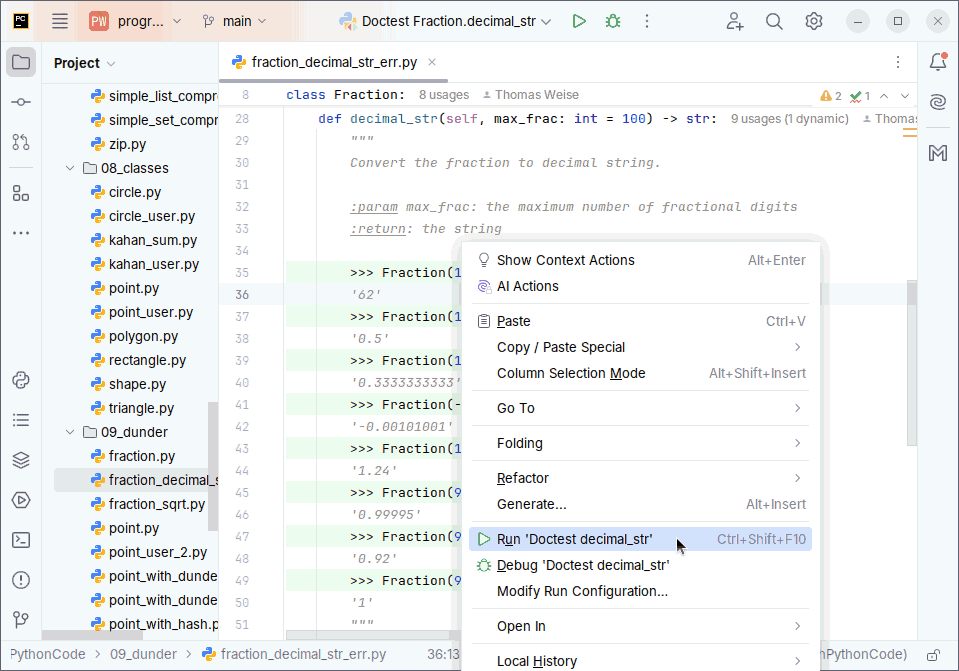
\includegraphics[width=0.48\linewidth]{\currentDir/doctests1}}}%
%
\floatSep%
%
\subfloat[][%
The \pglspl{doctest} are run, and in the window at the bottom-left, we see the failing tests.%
\label{fig:dunder:doctests2}%
]{\tightbox{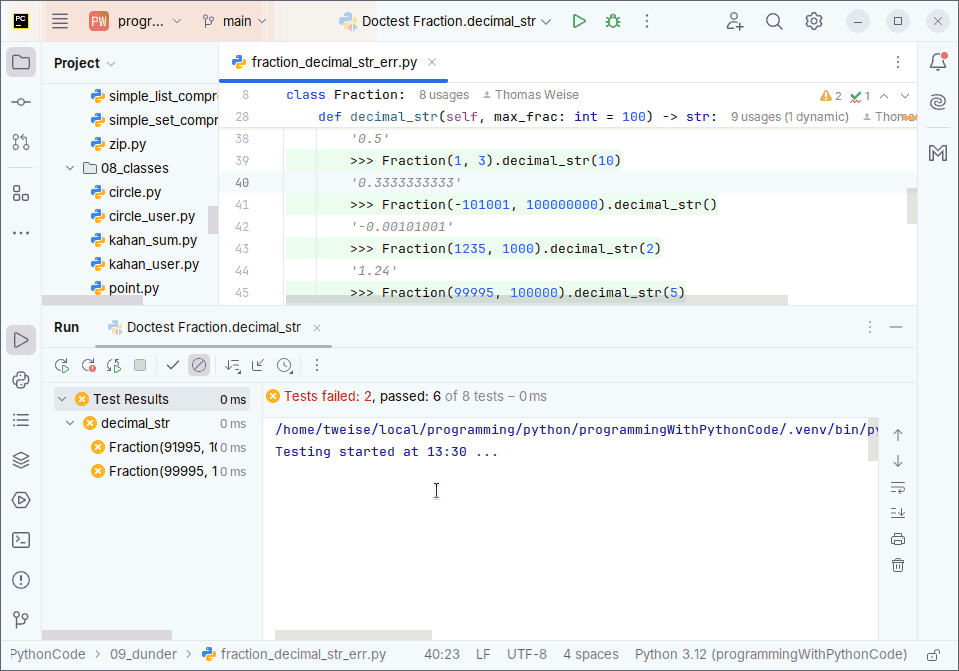
\includegraphics[width=0.48\linewidth]{\currentDir/doctests2}}}%
%
\floatRowSep%
%
\subfloat[][%
Left-clicking on the first failed test in the small window shows us the test output in bottom-centered window.%
\label{fig:dunder:doctests3}%
]{\tightbox{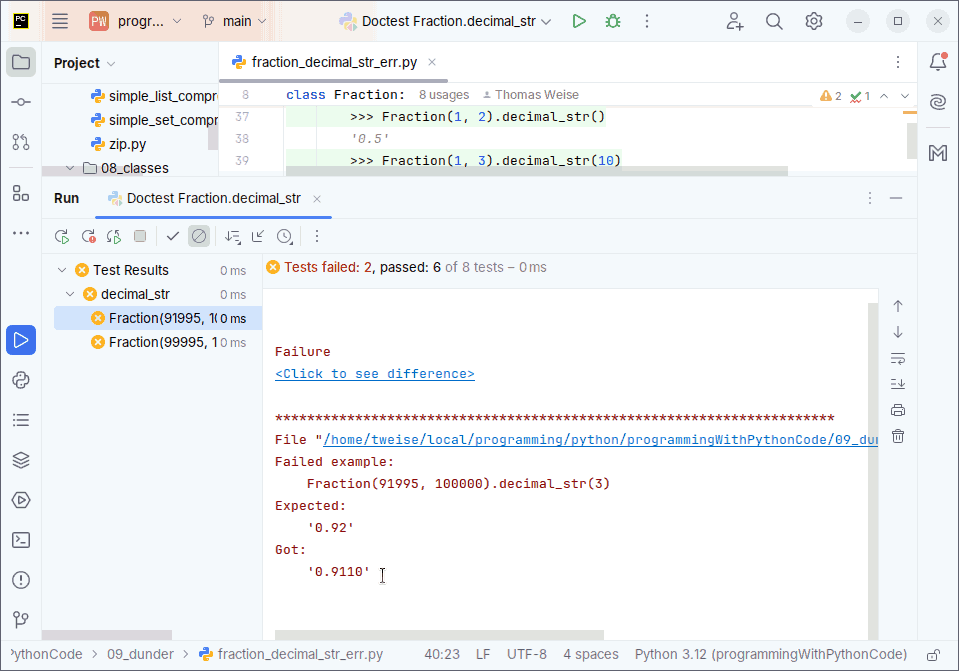
\includegraphics[width=0.48\linewidth]{\currentDir/doctests3}}}%
%
\floatSep%
%
\subfloat[][%
Left-clicking on the second failed test in the small window shows us the test output in bottom-centered window.%
\label{fig:dunder:doctests4}%
]{\tightbox{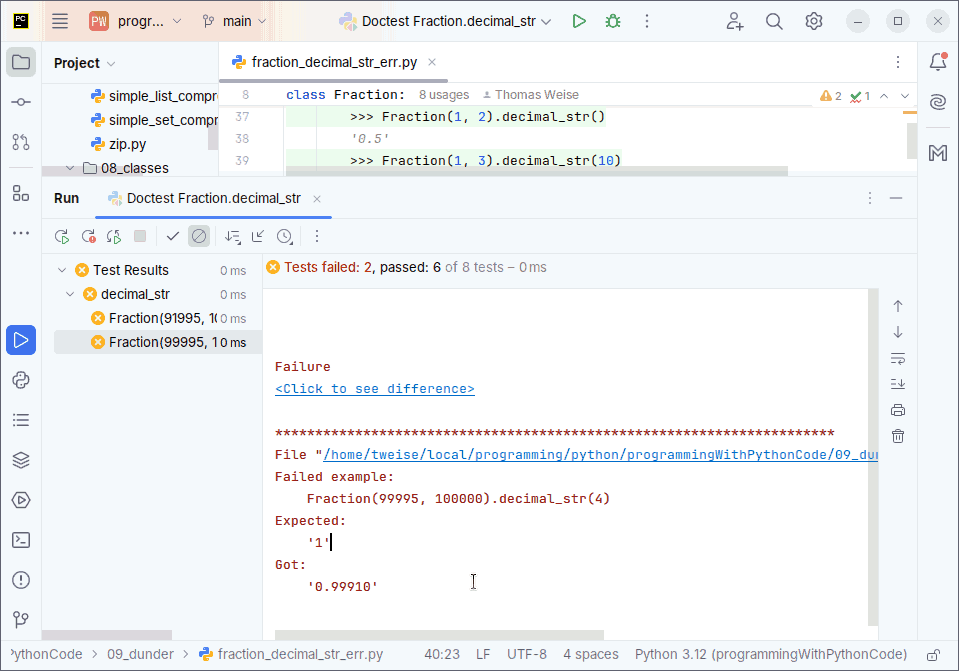
\includegraphics[width=0.48\linewidth]{\currentDir/doctests4}}}%%
%
\caption{Running \pglspl{doctest} in \pycharm.}%
\label{fig:dunder:doctests}%
\end{figure}%

We want to investigate this very strange error.
First, let us repeat the \pglspl{doctest} by also executing them inside \pycharm\ in \cref{fig:dunder:doctests}.
We open our source file and scroll to our function \pythonil{decimal_str}.
With a right mouse click, a context menu is opened.
Here, we then left-click on \menu{Run \inSQuotes{Doctest decimal\_str}}~(\cref{fig:dunder:doctests1}).

This executes \emph{all} the \pglspl{doctest}.
In the small window at the bottom-left, we can see the \emph{failing} tests~(\cref{fig:dunder:doctests2}).
We can click on these failed tests to get more information.
A left-click on the first failed test in this window in the bottom-left will then display the output of that text in the bottom-centered window~(\cref{fig:dunder:doctests3}).
This is the same information we already saw in \cref{exec:dunder:fraction_decimal_str_err:doctest}.
What we did not see in that output is that actually \emph{two} \pglspl{doctest} failed.
A left-click on the second failed test in~\cref{fig:dunder:doctests3} tells us that \pythonil{Fraction(99995, 100000).decimal_str(4)} did not yield the expected~\pythonil{"1"}.
Instead, it produced~\pythonil{"0.99910"}.
Why is there a \pythonil{"0"} at the end of our number?
Where did it come from?
Zeros at the end should not be possible with our code.
Also, there are four~9s in our number, not three.
What went wrong here?

We are clueless why these tests fail.
The question arises:
What can we do?

If we want to find where things go wrong, it would be very useful if we could somehow execute our program step-by-step.
When I explained how \pythonil{decimal_str} works, I used~$\frac{-179}{16}$ as an example and explained what the program would do.
Would it not be nice if we could actually step-by-step execute the program for the test and see what it \emph{actually} does?
Luckily, we can do that!
With a tool called \debugger\ which ships with \python\ and \pycharm.%
%
\usefulTool{debugger}{%
A \debugger\ is a tool that ships with many programming languages and \pglspl{ide}. %
It allows you to execute a program step-by-step while observing the current values of variables. %
This way, you can find errors in the code more easily~\cite{W2024PME,A2002D,R2007PPBPDTAM}. %
A comprehensive example on how to use the \debugger\ in \pycharm\ is given in~\cref{sec:dunder:debugging}.%
}%
%
\begin{figure}%
\centering%
%
\subfloat[][%
We open our source code file in \pycharm\ and locate our function \pythonil{decimal_str}.%
\label{fig:dunder:debug01}%
]{\tightbox{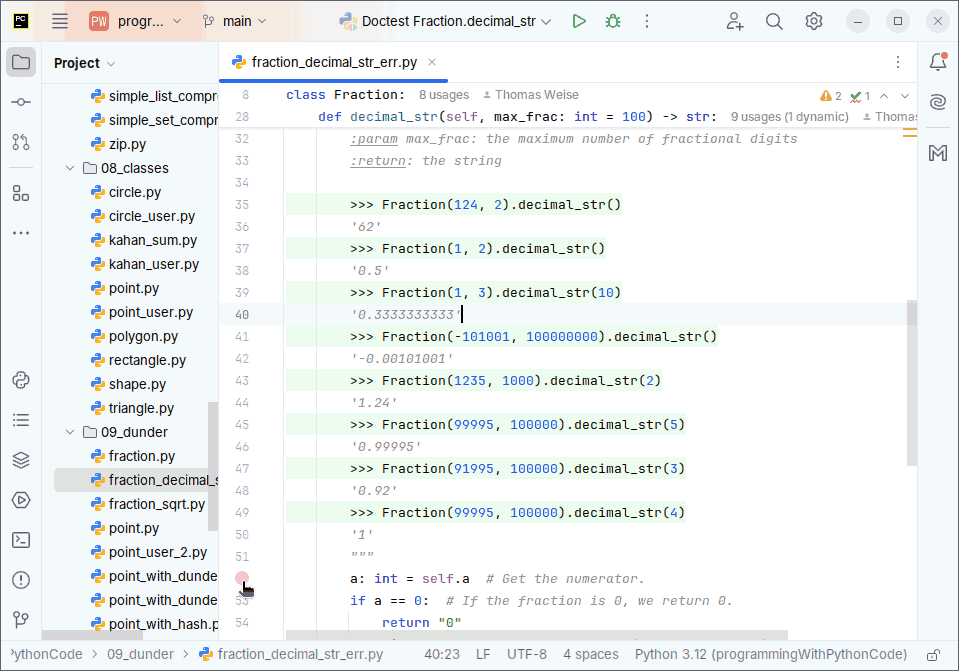
\includegraphics[width=0.48\linewidth]{\currentDir/debug01}}}%
%
\floatSep%
%
\subfloat[][%
We place a \pgls{breakpoint} at the first line of our function by right-clicking on the line number. %
This is denoted by the red ball over the line number. %
Later, the program execution will pause at this location.%
\label{fig:dunder:debug02}%
]{\tightbox{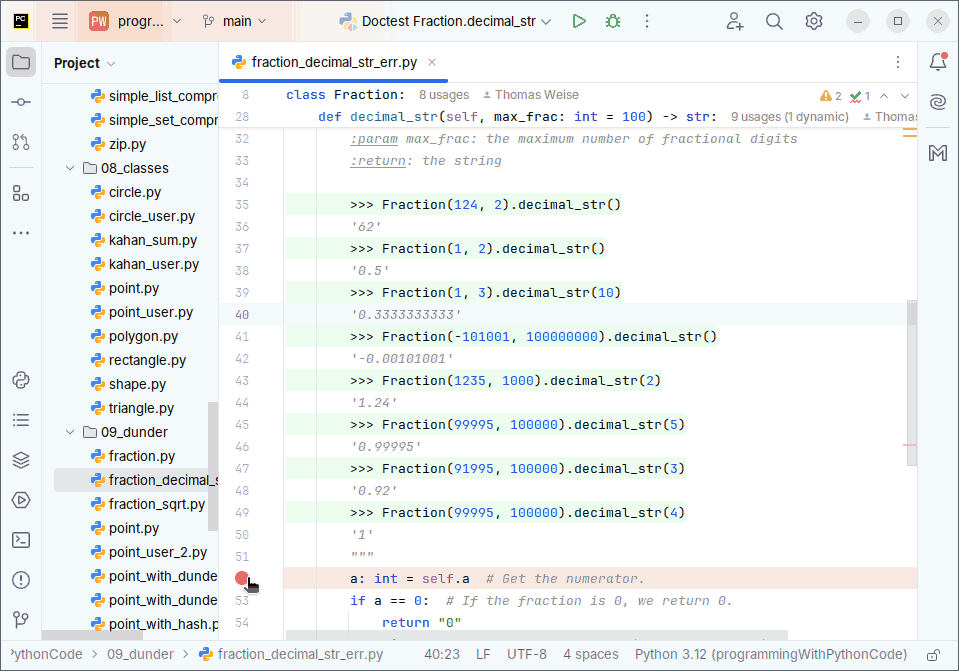
\includegraphics[width=0.48\linewidth]{\currentDir/debug02}}}%
%
\floatRowSep%
%
\subfloat[][%
We open the context menu by right-clicking into the \pgls{doctest} and click \menu{Debug \inSQuotes{Doctest decimal\_str}}.%
\label{fig:dunder:debug03}%
]{\tightbox{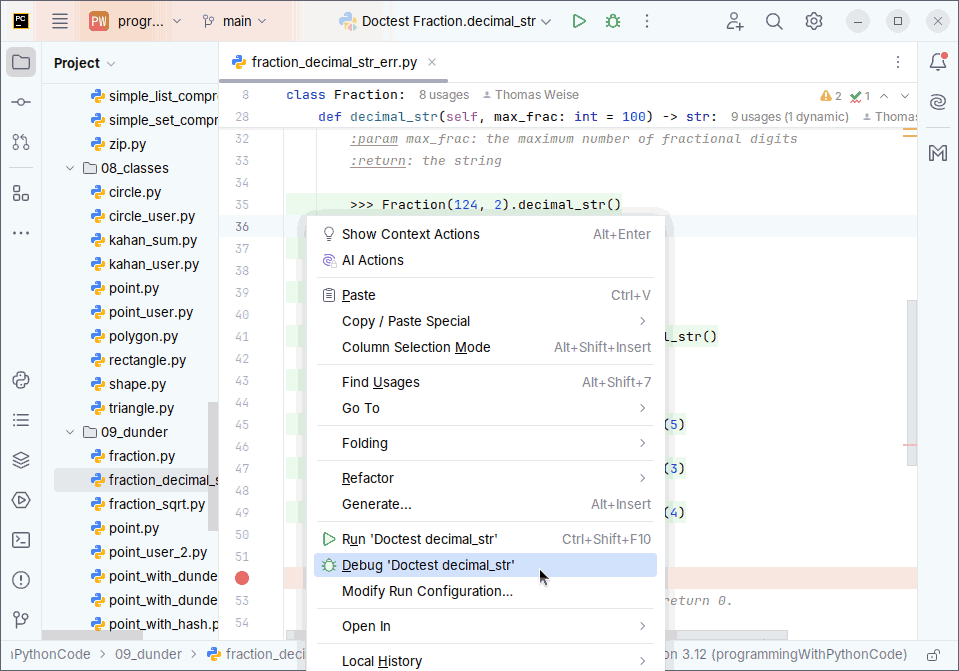
\includegraphics[width=0.48\linewidth]{\currentDir/debug03}}}%
%
\floatSep%
%
\subfloat[][%
The execution of the \pglspl{doctest} begins, but is immediately paused the first time the \pgls{breakpoint} is reached. %
This line is now marked with blue color, but not yet executed.%
\label{fig:dunder:debug04}%
]{\tightbox{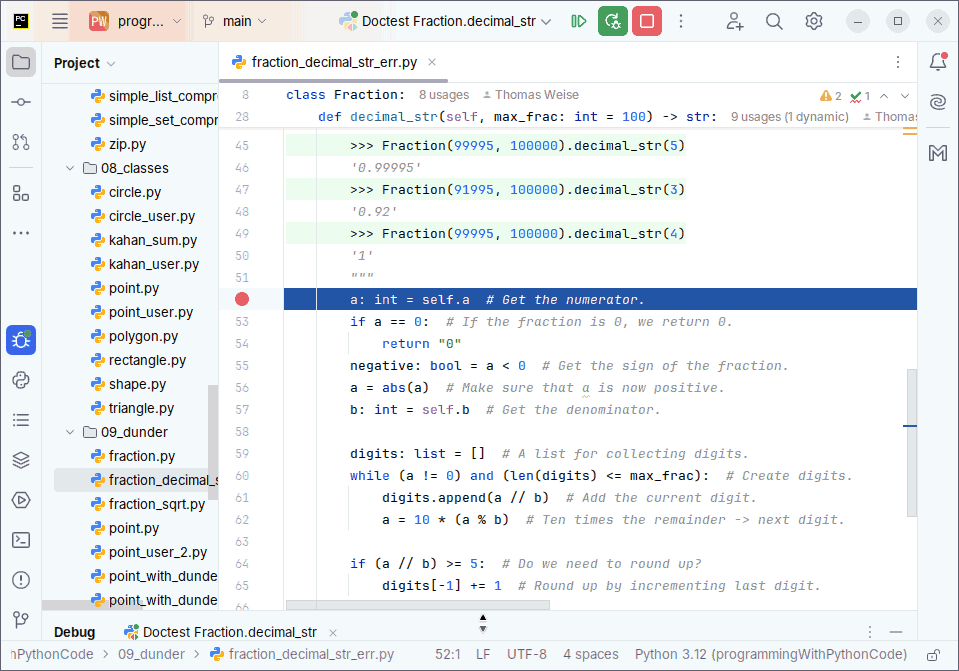
\includegraphics[width=0.48\linewidth]{\currentDir/debug04}}}%
%
\floatRowSep%
%
\subfloat[][%
We drag the \menu{Debug} register up from the bottom of our \pycharm\ window. %
We find the new register \menu{Threads \& Variables}, where we can see the value of all local variables at the current point in execution.%
\label{fig:dunder:debug05}%
]{\tightbox{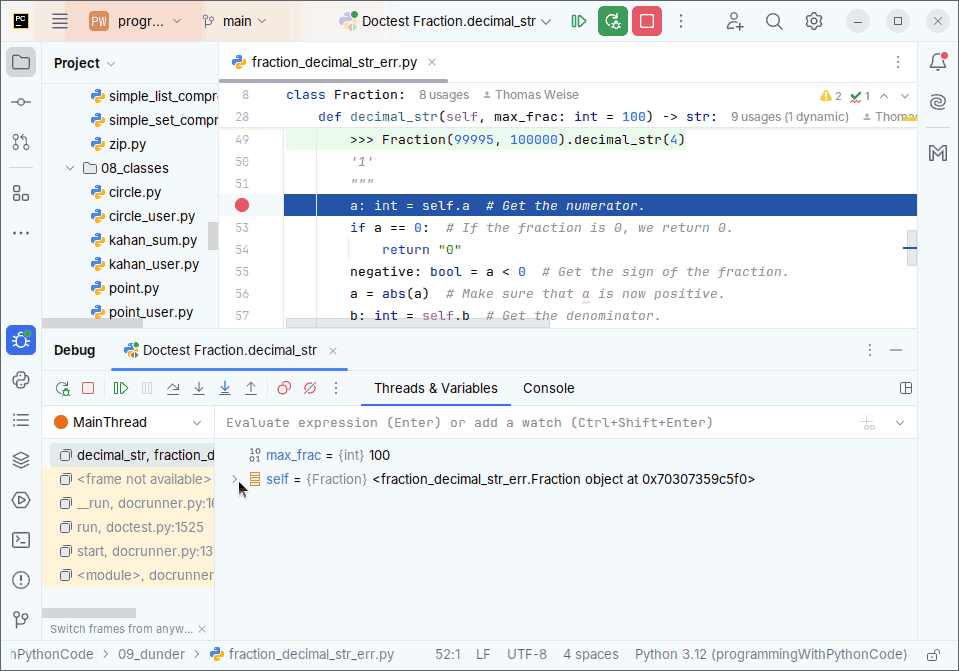
\includegraphics[width=0.48\linewidth]{\currentDir/debug05}}}%
%
\floatSep%
%
\subfloat[][%
Clicking on the variable \pythonil{self} reveals that we are in the first test case, where \pythonil{Fraction(124, 2)} is tested, which was normalized to \pythonil{Fraction(62, 1)} by the initializer~\pythonil{\_\_init\_\_}.%
\label{fig:dunder:debug06}%
]{\tightbox{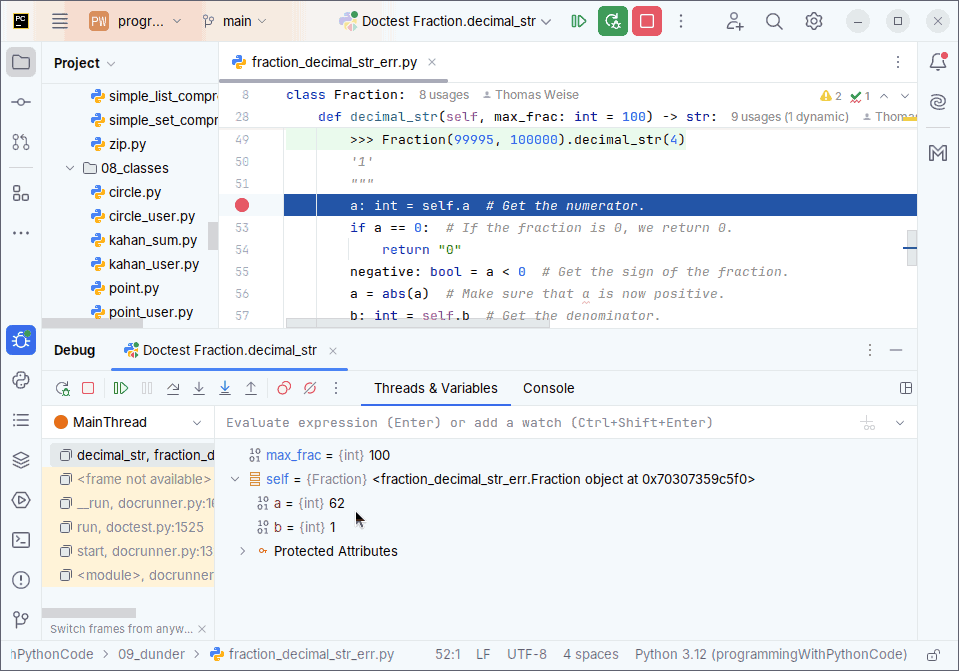
\includegraphics[width=0.48\linewidth]{\currentDir/debug06}}}%
%
\caption{Using the \debugger\ in \pycharm.}%
\label{fig:dunder:debugA}%
\end{figure}%
%
In \pycharm, we can apply the \debugger\ to a complete program, but also to \pglspl{doctest}.
This is what we will do in \cref{fig:dunder:debugA}.
First, we again open our program code in \pycharm\ and locate our function \pythonil{decimal_str}~(\cref{fig:dunder:debug01}).

On the left side of our code file, there is a column with the line numbers.
We can left-click on a line to place a \pgls{breakpoint} there.
A \pgls{breakpoint} is a mark in the \pgls{ide} at which we later want the program execution to pause.
We want our program to pause right at the beginning of \pythonil{decimal_str}, so be place the \pgls{breakpoint} there~(\cref{fig:dunder:debug02}).
The \pgls{breakpoint} is shown as a red ball over the line number.

In order to begin the debugging process, we again open the context menu by right-clicking into the \pgls{doctest}.
This time, instead of \emph{running} the \pgls{doctest}, we click \menu{Debug \inSQuotes{Doctest decimal\_str}}~(\cref{fig:dunder:debug03}).
The \pglspl{doctest} will now be executed, but instead of running them completely, the \pgls{debugger} kicks in:
The execution is paused at exactly our \pgls{breakpoint}.
This line of code is \emph{not yet executed}, but marked in blue~(\cref{fig:dunder:debug04}).

Before we continue, we look at the bottom of our \pycharm\ window.
There is a row with a \menu{Debug} register.
We can right-click the top of this row and drag it upwards.
Now we get a division of our window that contains the debug information.
Most importantly, in the register \menu{Threads \& Variables}, we can see the values of all local variables at the current point in execution~(\cref{fig:dunder:debug05}).

We see that \pythonil{max_frac} has the value \pythonil{100}.
When clicking on the variable \pythonil{self}, we see that the \pgls{numerator}~\pythonil{a} of the current fraction has value~\pythonil{62}, while the \pgls{denominator}~\pythonil{b} is~\pythonil{1}.
This is exactly what we expect:
Our first test case was \pythonil{Fraction(124, 2).decimal_str()}, so the normalized fraction is indeed~$\frac{62}{1}$.%
%
\clearpage%
\begin{figure}%
\ContinuedFloat%
\centering%
%
\subfloat[][%
The first \pgls{doctest} case~$\frac{124}{2}$ is uninteresting, so we continue the program execution by clicking \pycharmDebuggerResume\ or hitting \keys{F9}.%
\label{fig:dunder:debug07}%
]{\tightbox{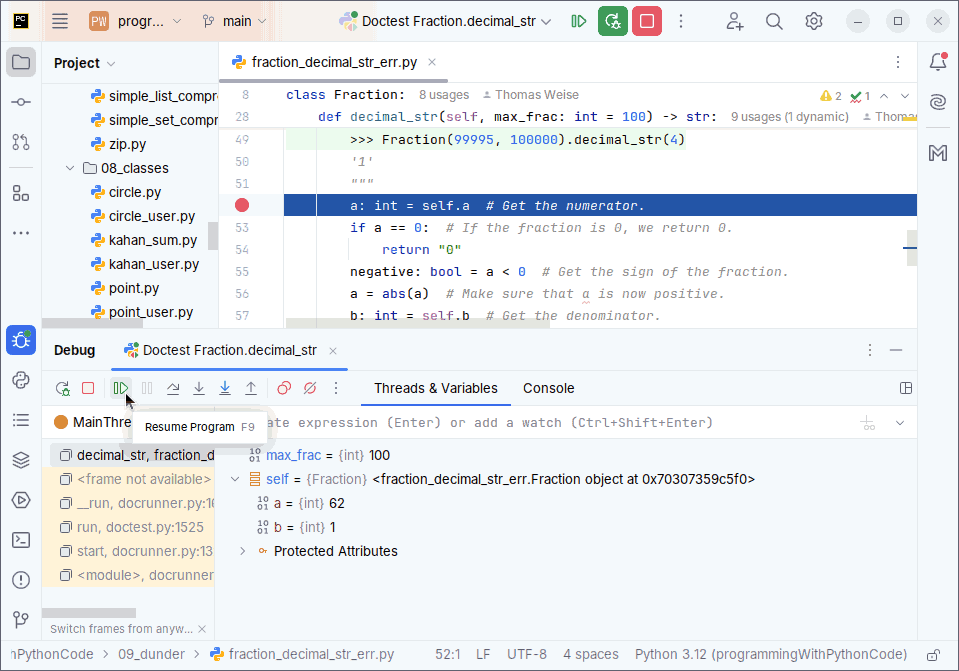
\includegraphics[width=0.48\linewidth]{\currentDir/debug07}}}%
%
\floatSep%
%
\subfloat[][%
The second \pgls{doctest} case~$\frac{1}{2}$ is also uninteresting. %
We continue the program execution by clicking \pycharmDebuggerResume.%
\label{fig:dunder:debug08}%
]{\tightbox{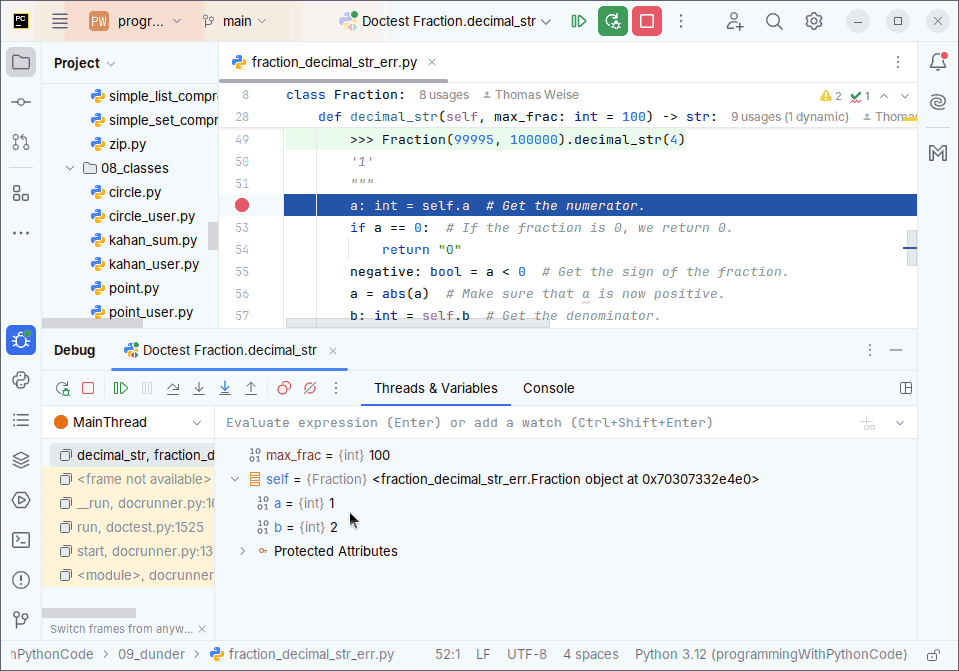
\includegraphics[width=0.48\linewidth]{\currentDir/debug08}}}%
%
\floatRowSep%
%
\subfloat[][%
The third \pgls{doctest} case, where the fraction is~$\frac{1}{3}$ and \pythonil{max_frac} is~\pythonil{10}. %
We again skip over it by pressing~\keys{F9}.%
\label{fig:dunder:debug09}%
]{\tightbox{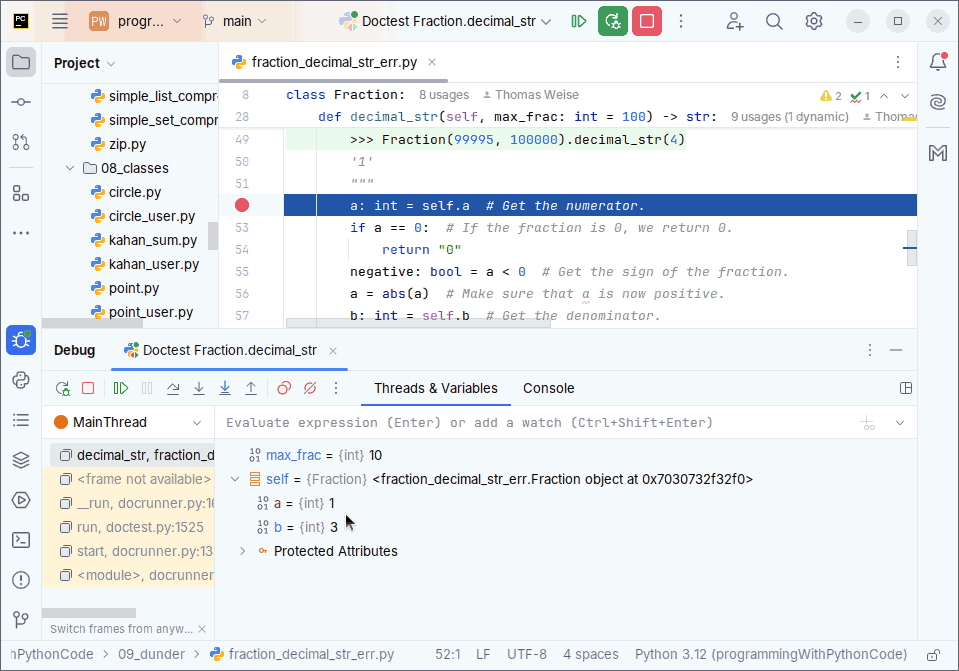
\includegraphics[width=0.48\linewidth]{\currentDir/debug09}}}%
%
\floatSep%
%
\subfloat[][%
The fourth \pgls{doctest} case~$\frac{-101001}{100000000}$ can be skipped as well.%
\label{fig:dunder:debug10}%
]{\tightbox{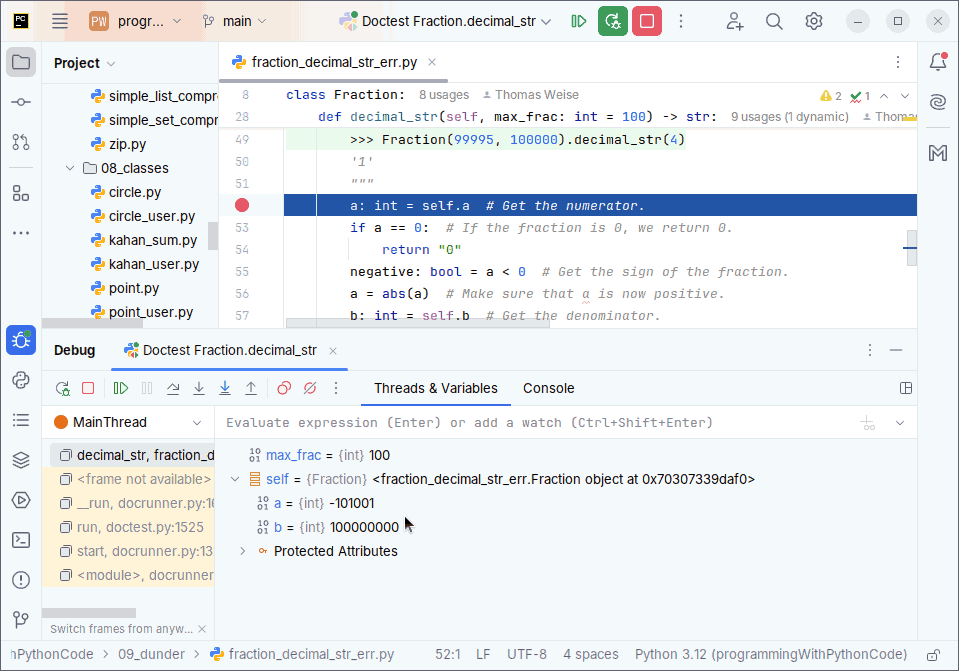
\includegraphics[width=0.48\linewidth]{\currentDir/debug10}}}%
%
\floatRowSep%
%
\subfloat[][%
The test case~$\frac{1235}{1000}$, normalized to~$\frac{247}{200}$, also was successful and can be skipped by pressing~\pycharmDebuggerResume.%
\label{fig:dunder:debug11}%
]{\tightbox{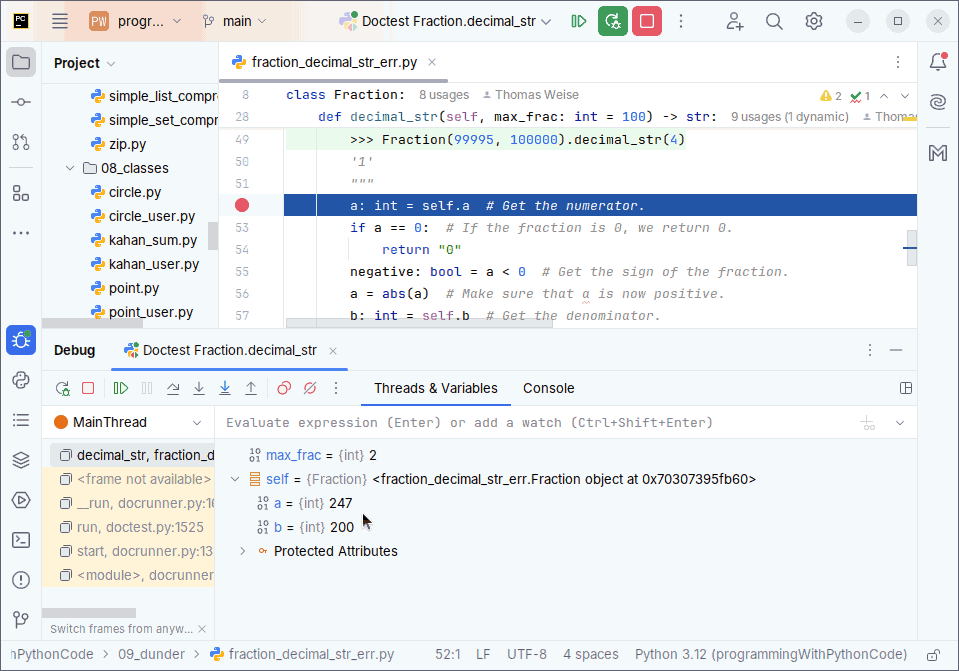
\includegraphics[width=0.48\linewidth]{\currentDir/debug11}}}%
%
\floatSep%
%
\subfloat[][%
The last one of the uninteresting \pgls{doctest} cases:~\pythonil{Fraction(99995, 100000)}. %
We again press~\keys{F9}.%
\label{fig:dunder:debug12}%
]{\tightbox{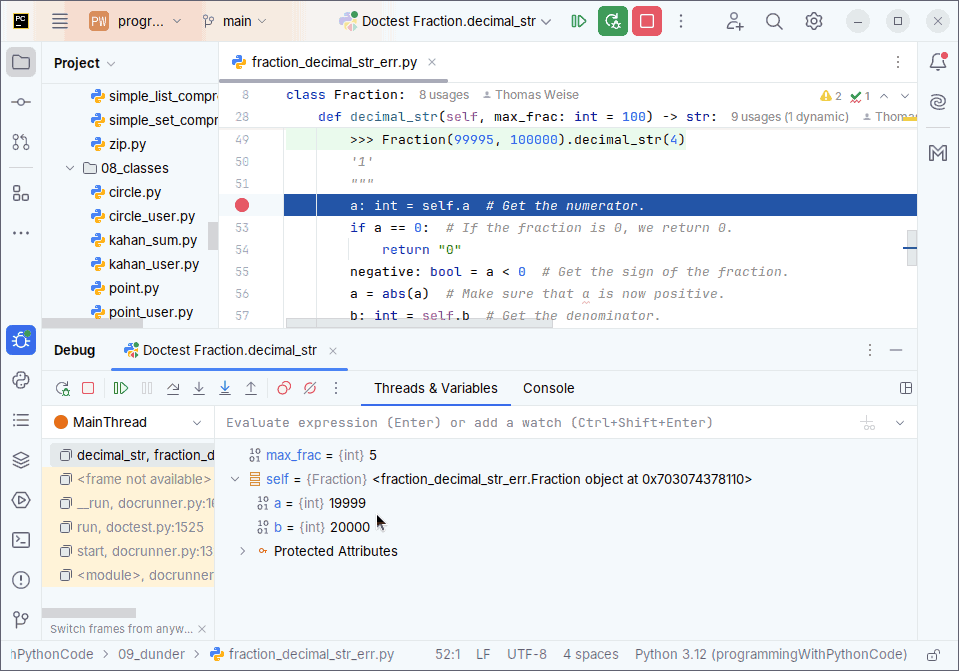
\includegraphics[width=0.48\linewidth]{\currentDir/debug12}}}%
%
\caption{Using the \debugger\ in \pycharm~(continued).}%
\label{fig:dunder:debugB}%
\end{figure}%

This test case is already successful, so we are not interested in it.
Among the symbols in \menu{Debug} register, we click \pycharmDebuggerResume, which will let the program continue its execution~(\cref{fig:dunder:debug07}).
Alternatively, we can hit \keys{F9}, which has the same effect.
The execution of the \pglspl{doctest} is resumed, but again pauses at our \pgls{breakpoint}~(\cref{fig:dunder:debug08}).
This time, we can see that we have arrived at the beginning of the second \pgls{doctest} case with \pythonil{Fraction(1, 2)}.
We again continue by clicking \pycharmDebuggerResume\ or pressing~\keys{F9}.
This takes us to the beginning of the third \pgls{doctest} case, where the fraction is~$\frac{1}{3}$ and \pythonil{max_frac} is~\pythonil{10}~(\cref{fig:dunder:debug09}).
We can skip it as well by pressing~\keys{F9}.
The next time we reach the \pgls{breakpoint} is for the fourth \pgls{doctest} case, $\frac{-101001}{100000000}$~(\cref{fig:dunder:debug10}), which we skip, too.
When the debugger arrives at the fifth test case, \pythonil{Fraction(1235, 1000)}, we find that this fraction has been normalized correctly to~$\frac{247}{200}$.
Nonetheless, we can skip this test case via \keys{F9}, too, because we know that it will succeed~(\cref{fig:dunder:debug11}).
This takes us to the last successful \pgls{doctest} case, \pythonil{Fraction(99995, 100000)}, which corresponds to~$\frac{19999}{20000}$ in \cref{fig:dunder:debug12}.
After skipping it by pressing~\pycharmDebuggerResume, we will finally arrive at the cases that did fail and which we hence want to investigate step-by-step.

\begin{figure}%
\ContinuedFloat%
\centering%
%
\subfloat[][%
We arrive at the beginning of the failing \pgls{doctest} case \pythonil{Fraction(91995, 100000).decimal_str(3)}. %
The \pythonil{max_frac} parameter has value~\pythonil{3}, \pythonil{self.a} is \pythonil{18399} and \pythonil{self.b} is \pythonil{20000}, because the fraction was normalized in \pythonil{\_\_init\_\_}.%
\label{fig:dunder:debug13}%
]{\tightbox{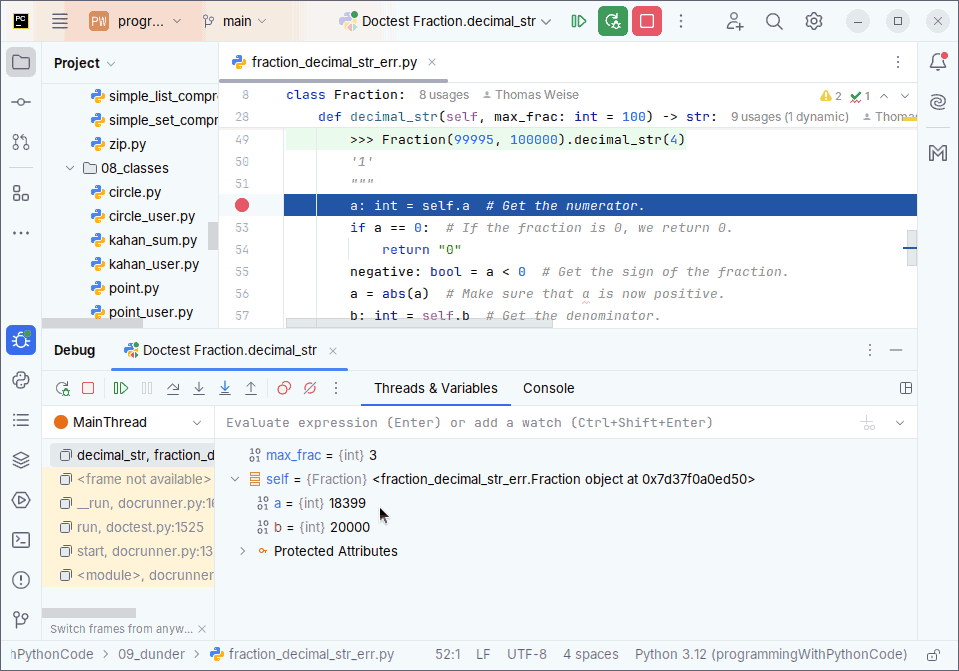
\includegraphics[width=0.48\linewidth]{\currentDir/debug13}}}%
%
\floatSep%
%
\subfloat[][%
We now execute the first line of the \pythonil{decimal_str} function where the \pgls{debugger} has paused. %
This is done by either pressing the \pycharmDebuggerStepOver~button or by hitting~\keys{F8}.%
\label{fig:dunder:debug14}%
]{\tightbox{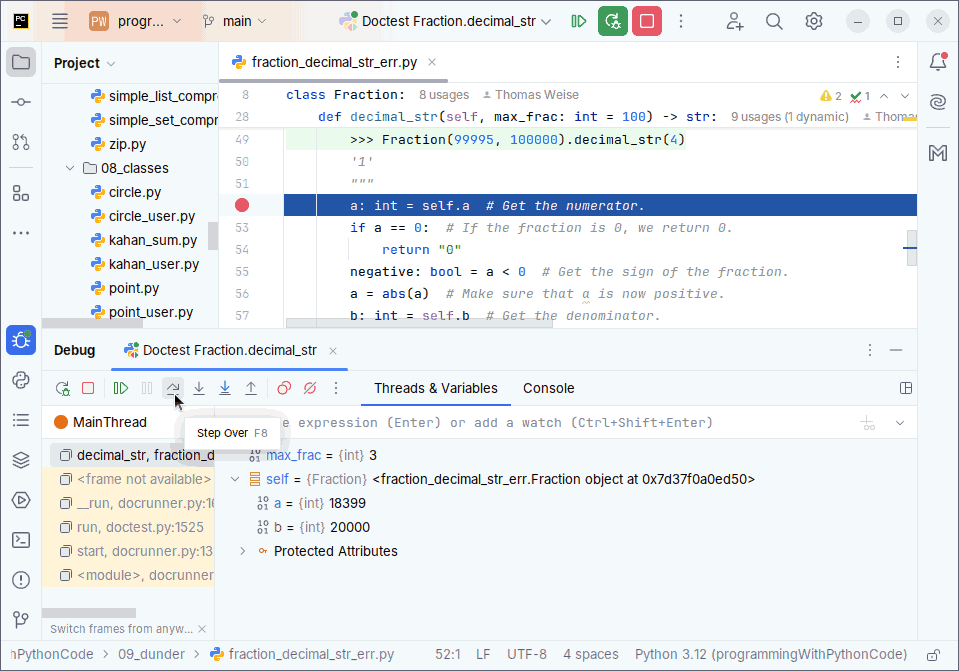
\includegraphics[width=0.48\linewidth]{\currentDir/debug14}}}%
%
\floatRowSep%
%
\subfloat[][%
The execution of the assignment \pythonil{a = self.a} creates a new local variable~\pythonil{a} with value~\pythonil{18399}. %
We press \keys{F8} to continue the execution.%
\label{fig:dunder:debug15}%
]{\tightbox{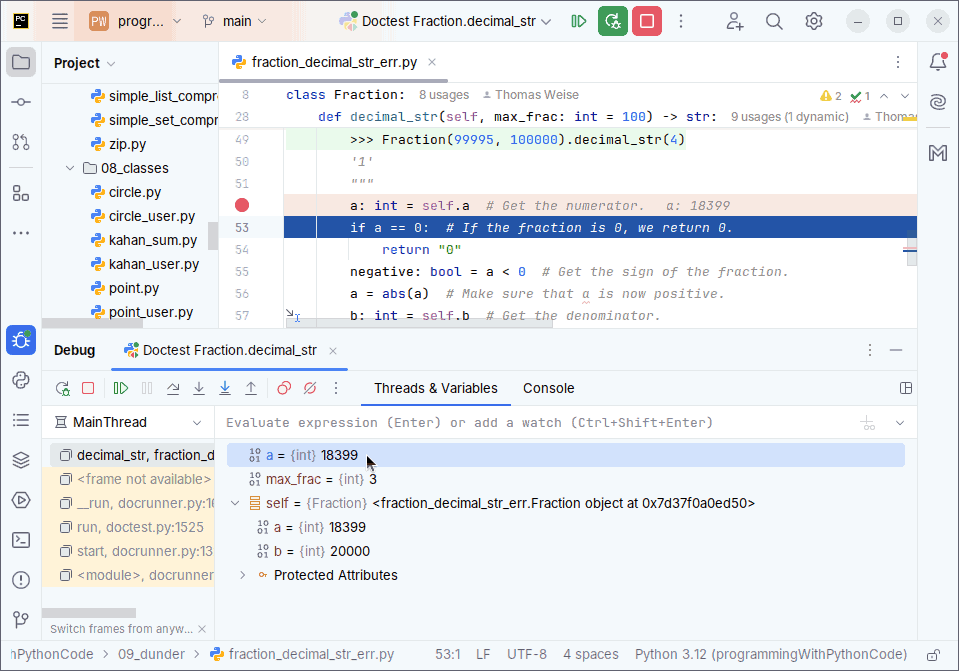
\includegraphics[width=0.48\linewidth]{\currentDir/debug15}}}%
%
\floatSep%
%
\subfloat[][%
The condition for the \pythonil{if} is not met, so the execution jumps over its body and the next line after the \pythonil{if} is marked. %
We execute it by pressing~\pythonil{F8}.%
\label{fig:dunder:debug16}%
]{\tightbox{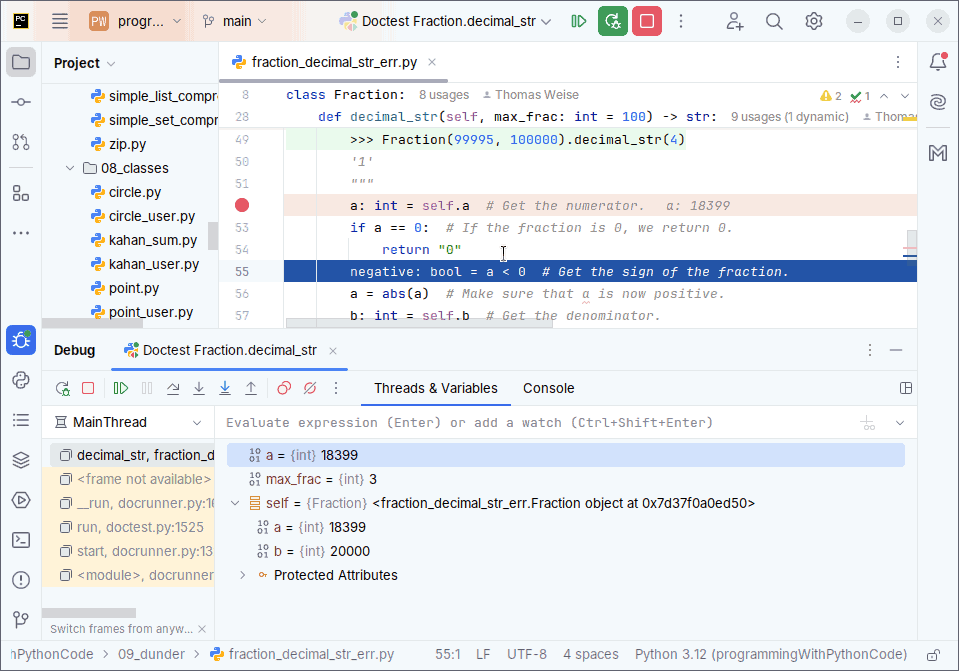
\includegraphics[width=0.48\linewidth]{\currentDir/debug16}}}%
%
\floatRowSep%
%
\subfloat[][%
The new local variable~\pythonil{negative} with value~\pythonil{False} appears. %
The next line of code is marked and we execute it by pressing~\pycharmDebuggerStepOver.%
\label{fig:dunder:debug17}%
]{\tightbox{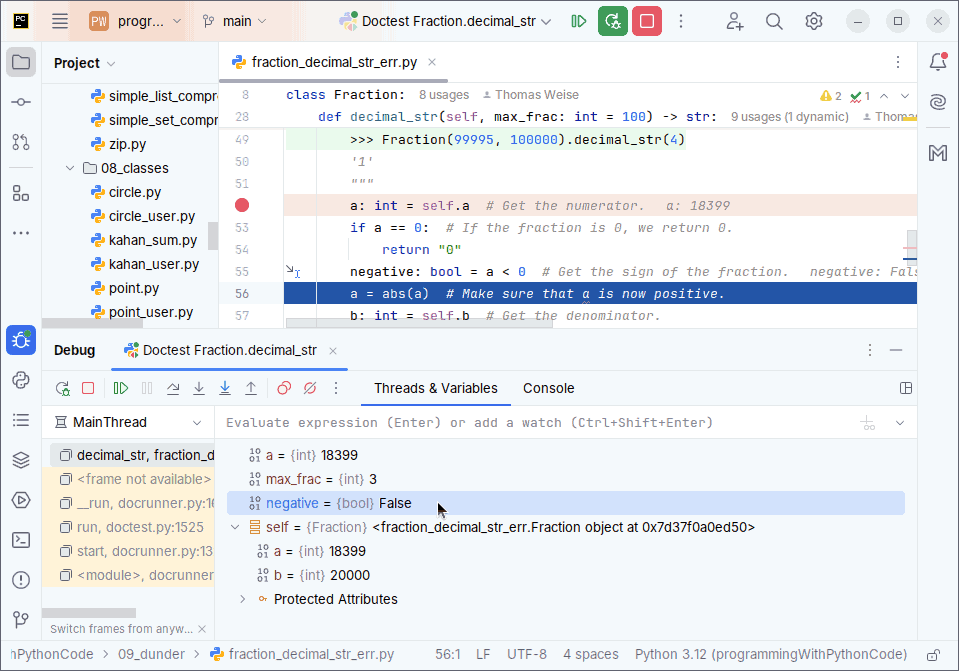
\includegraphics[width=0.48\linewidth]{\currentDir/debug17}}}%
%
\floatSep%
%
\subfloat[][%
\pythonil{a = abs(a)} has no effect, since \pythonil{a} is already positive.
We press \keys{F8} to continue.%
\label{fig:dunder:debug18}%
]{\tightbox{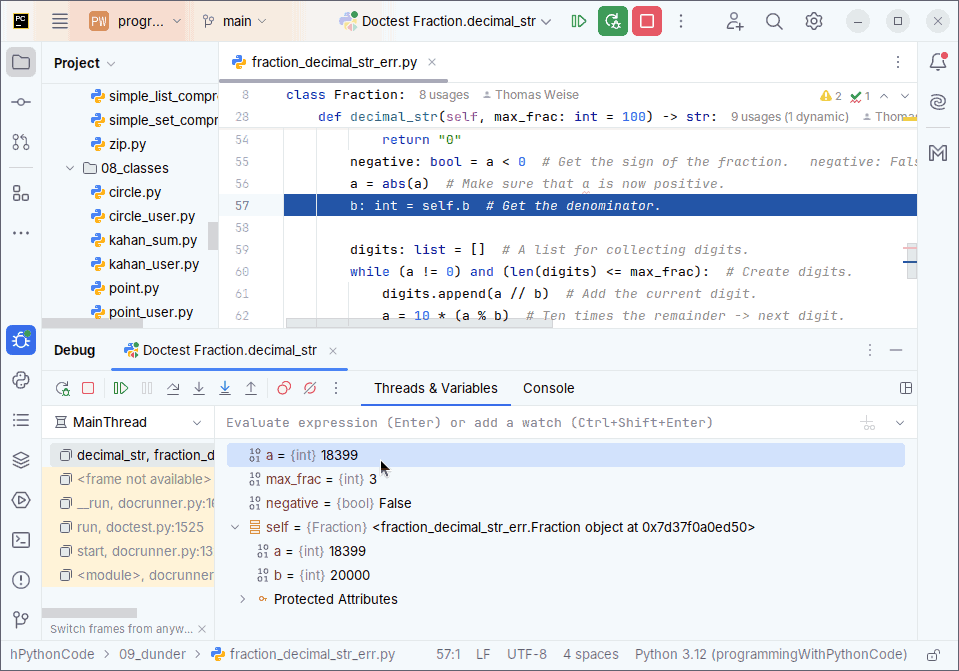
\includegraphics[width=0.48\linewidth]{\currentDir/debug18}}}%
%
%
\caption{Using the \debugger\ in \pycharm~(continued).}%
\label{fig:dunder:debugC}%
\end{figure}%
%
\begin{sloppypar}%
\Cref{fig:dunder:debug13} shows that we now arrived at the beginning of the failing \pgls{doctest} case \pythonil{Fraction(91995, 100000).decimal_str(3)}.
The fraction~$\frac{91995}{100000}$ got normalized to~$\frac{18399}{20000}$ in the initializer~\pythonil{\_\_init\_\_}.
The parameter \pythonil{max_frac} of \pythonil{decimal_str} has the value~\pythonil{3}, as we can see in the \menu{Threads \& Variables} window.
We now want to execute the \pythonil{decimal_str} method step-by-step.
Right now, the \pgls{debugger} has paused the execution right at the very first line of this function.
This line has not yet been executed.%
\end{sloppypar}%
%
In \cref{fig:dunder:debug14}, we execute this line of code, either by pressing the \pycharmDebuggerStepOver~button or by hitting~\keys{F8}.
We can see in \cref{fig:dunder:debug15} that now a new variable has appeared in the \menu{Threads \& Variables} window.
Since we executed \pythonil{a = self.a}, the local variable~\pythonil{a} now exists and has value~\pythonil{18399}.
Now, the next line of code that can be executed is marked with blue color.

By pressing \keys{F8}, the \pythonil{if a == 0:} is executed.
Since \pythonil{a == 0} is not \pythonil{True}, the body of the \pythonil{if} is not executed.
The program jumps right over it.
The next line after the \pythonil{if} is marked~\cref{fig:dunder:debug16}.
We execute it by pressing~\keys{F8}.

The local variable \pythonil{negative} is created.
Since \pythonil{a < 0} is \pythonil{False}, \pythonil{negative} is \pythonil{False}, too.
The next line of code is marked and we press~\pycharmDebuggerStepOver\ to execute it~(\cref{fig:dunder:debug17}).

\pythonil{a = abs(a)} has no effect, since \pythonil{a} is already positive.
We press \keys{F8} to continue~(\cref{fig:dunder:debug18}).
\clearpage%
%
\begin{figure}%
\ContinuedFloat%
\centering%
%
\subfloat[][%
After executing \pythonil{b = self.b}, the new local variable \pythonil{b} with value \pythonil{20000} comes into existence. %
We continue debugging by pressing~\keys{F8}.%
\label{fig:dunder:debug19}%
]{\tightbox{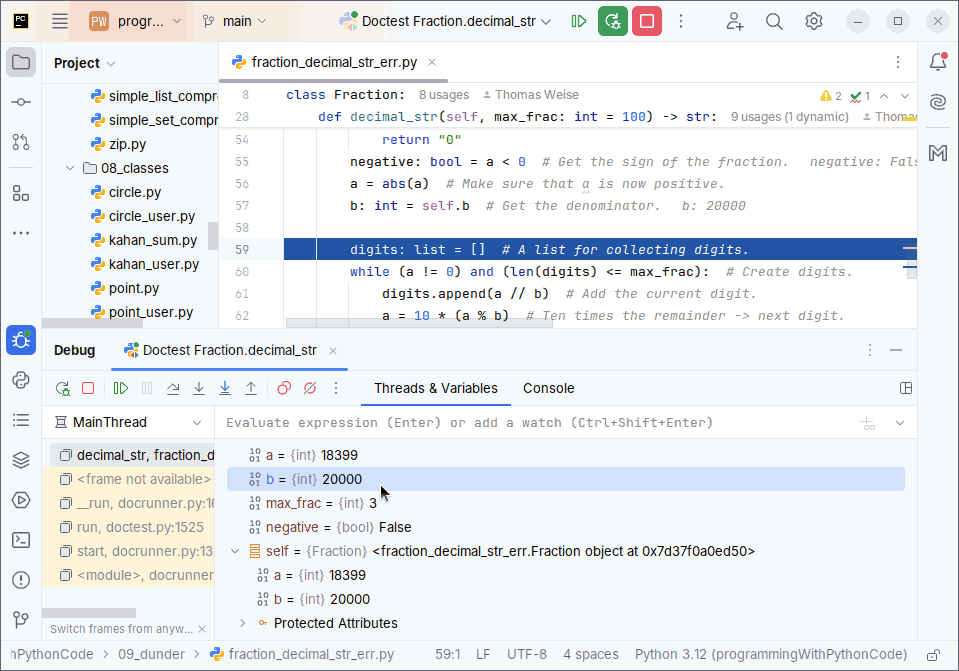
\includegraphics[width=0.48\linewidth]{\currentDir/debug19}}}%
%
\floatSep%
%
\subfloat[][%
The empty list \pythonil{digits} has been created. %
By pressing~\keys{F8}, the executing \pythonil{while} loop will begin by checking its condition.%
\label{fig:dunder:debug20}%
]{\tightbox{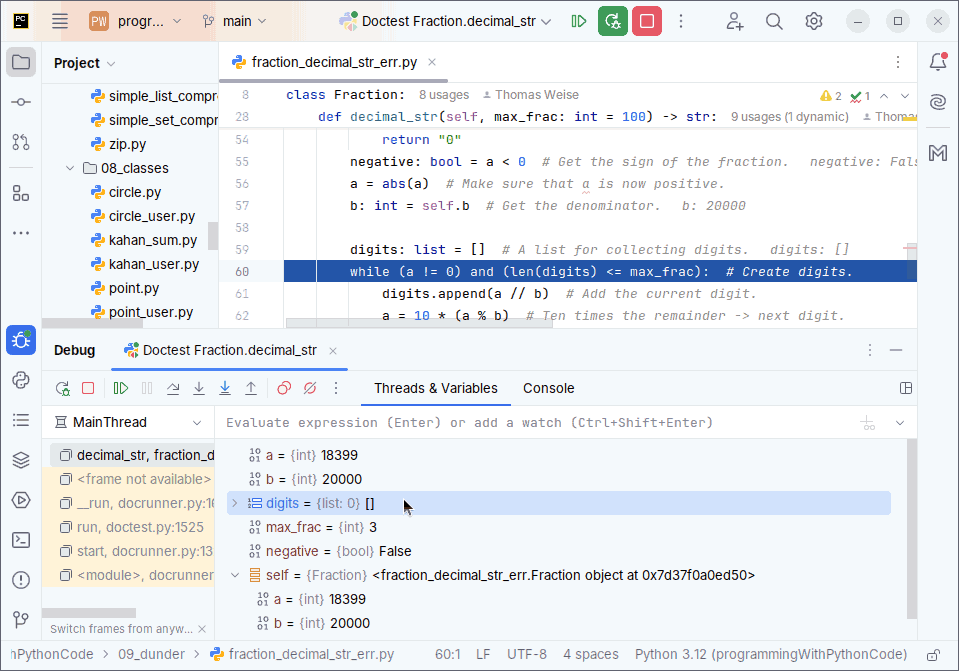
\includegraphics[width=0.48\linewidth]{\currentDir/debug20}}}%
%
\floatRowSep%
%
\subfloat[][%
The condition of the \pythonil{while} loop is met. %
The first line of the loop's body is marked. %
We press~\pycharmDebuggerStepOver\ to execute it.%
\label{fig:dunder:debug21}%
]{\tightbox{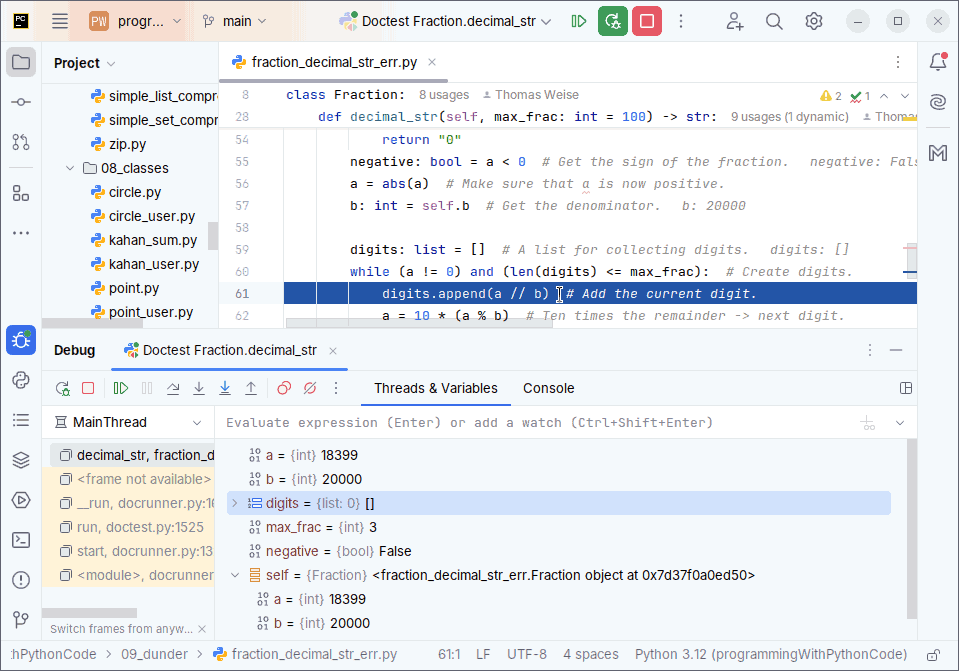
\includegraphics[width=0.48\linewidth]{\currentDir/debug21}}}%
%
\floatSep%
%
\subfloat[][%
\pythonil{digits} now contains the result of \pythonil{a // b}, i.e., is~\pythonil{[0]}. %
We press~\keys{F8}.%
\label{fig:dunder:debug22}%
]{\tightbox{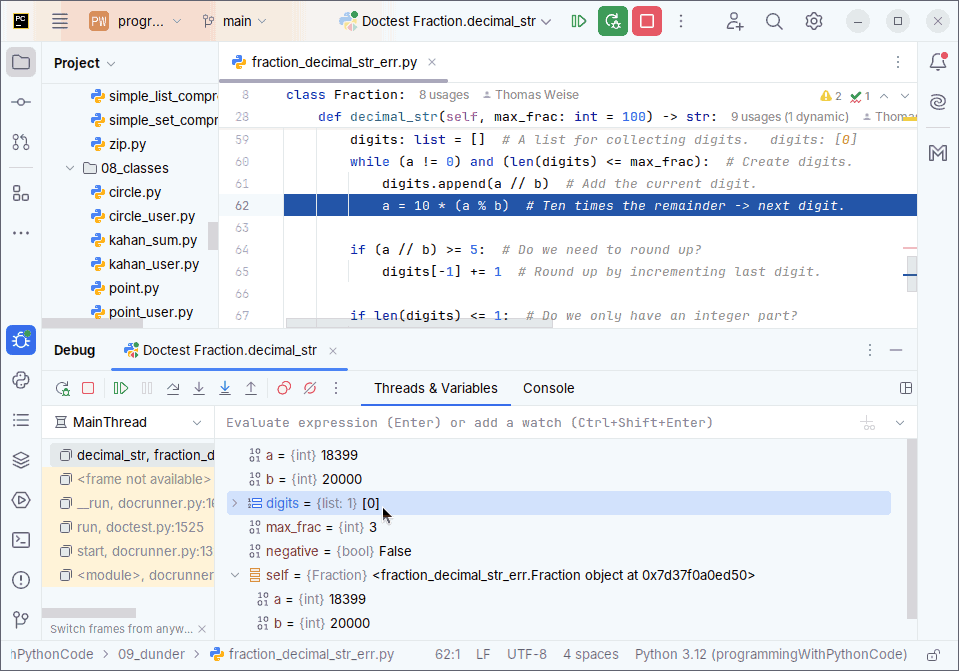
\includegraphics[width=0.48\linewidth]{\currentDir/debug22}}}%
%
\floatRowSep%
%
\subfloat[][%
\pythonil{a} now is \pythonil{183990}. %
We press~\pycharmDebuggerStepOver\ to continue.%
\label{fig:dunder:debug23}%
]{\tightbox{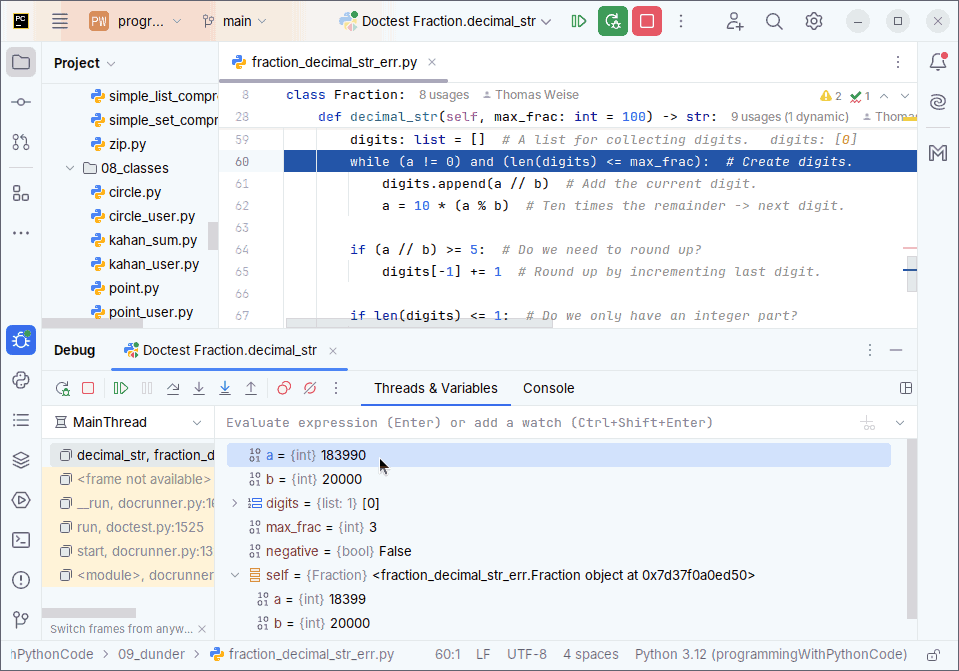
\includegraphics[width=0.48\linewidth]{\currentDir/debug23}}}%
%
\floatSep%
%
\subfloat[][%
We hit the \keys{F8} key to continue. %
The loop condition is still met, so the first line of the loop body is marked again.%
\label{fig:dunder:debug24}%
]{\tightbox{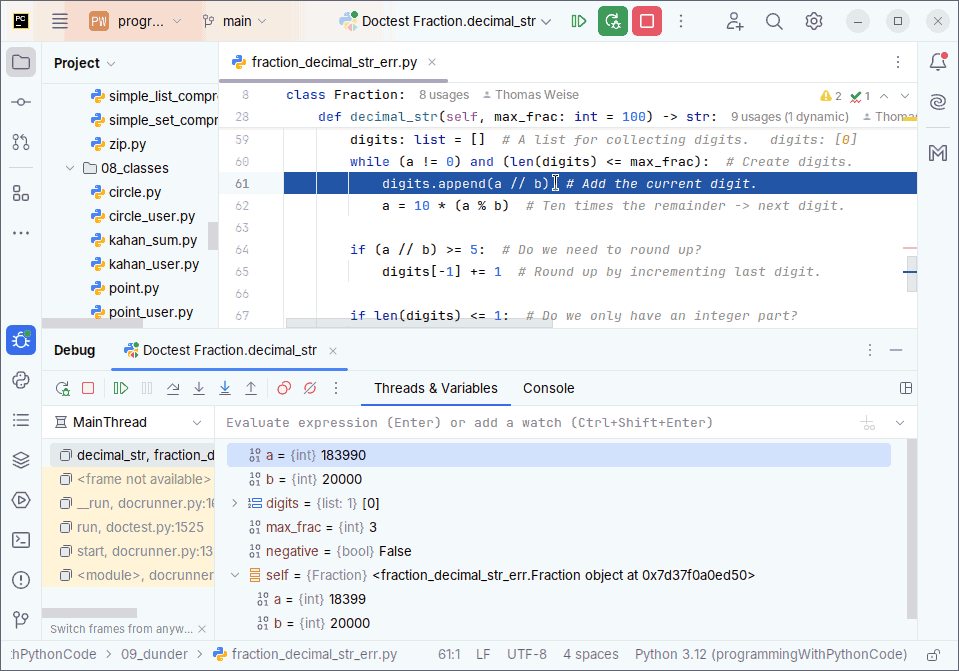
\includegraphics[width=0.48\linewidth]{\currentDir/debug24}}}%
%
\caption{Using the \debugger\ in \pycharm~(continued).}%
\label{fig:dunder:debugD}%
\end{figure}%

This executes \pythonil{b = self.b}.
Thus, the new local variable \pythonil{b} with value \pythonil{20000} is created in~\cref{fig:dunder:debug19}.
We are now at the last line of \inQuotes{trivial setup} of our \pythonil{decimal_str} method, the creation of the list~\pythonil{digits}.
We continue debugging by pressing~\keys{F8}.

The new variable~\pythonil{digits} has indeed appeared in~\cref{fig:dunder:debug20}.
It is an empty list~\pythonil{[]}.
We arrived at the beginning the \pythonil{while} loop.
We press \keys{F8}, which will cause the condition of the loop being checked.

In \cref{fig:dunder:debug21}, we find that now the first line of the loop's body is marked.
This means that \pythonil{a != 0} and \pythonil{len(digits) <= max_frac} are both~\pythonil{True}.
And they should be, since \pythonil{a} is \pythonil{18399}, \pythonil{len(digits)} if~0, and \pythonil{max_frac} is~3.
We press the \pycharmDebuggerStepOver~button to execute the first line of the loop body.

\pythonil{digits.append(a // b)} will append the value \pythonil{18399 // 20000} to the list~\pythonil{digits}.
As this is the result of an integer division where the \pgls{denominator} is larger than the \pgls{numerator}, \pythonil{digits} is now~\pythonil{[0]}~(\cref{fig:dunder:debug22}).
We press \keys{F8} to continue.

Now, \pythonil{a = 10 * (a \% b)} is executed.
Since \pythonil{18399 \% 20000} is still \pythonil{18399}, \pythonil{a} becomes \pythonil{183990} in \cref{fig:dunder:debug23}.
The head of the loop is now marked again.
We press the \pycharmDebuggerStepOver~button to let execute it.

In \cref{fig:dunder:debug24}, we again hit \keys{F8}.
The loop condition is still met, so the first line in the loop body is marked again.

\begin{figure}%
\ContinuedFloat%
\centering%
%
\subfloat[][%
\pythonil{9} gets appended to \pythonil{digits}.%
\label{fig:dunder:debug25}%
]{\tightbox{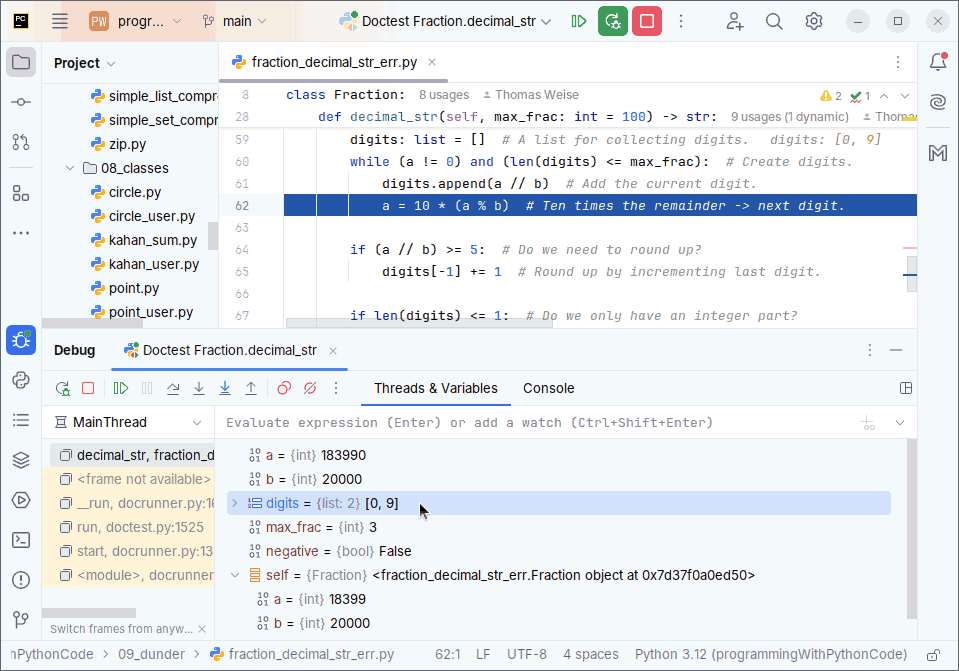
\includegraphics[width=0.48\linewidth]{\currentDir/debug25}}}%
%
\floatSep%
%
\subfloat[][%
\pythonil{a} gets updated to \pythonil{39900}.%%
\label{fig:dunder:debug26}%
]{\tightbox{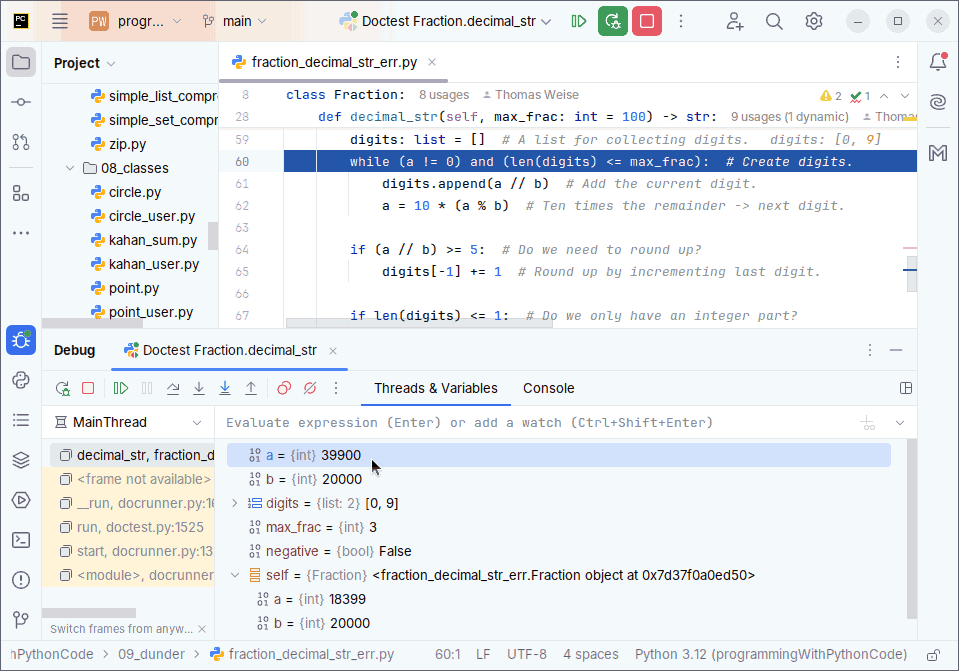
\includegraphics[width=0.48\linewidth]{\currentDir/debug26}}}%
%
\floatRowSep%
%
\subfloat[][%
The loop condition is still met.%
\label{fig:dunder:debug27}%
]{\tightbox{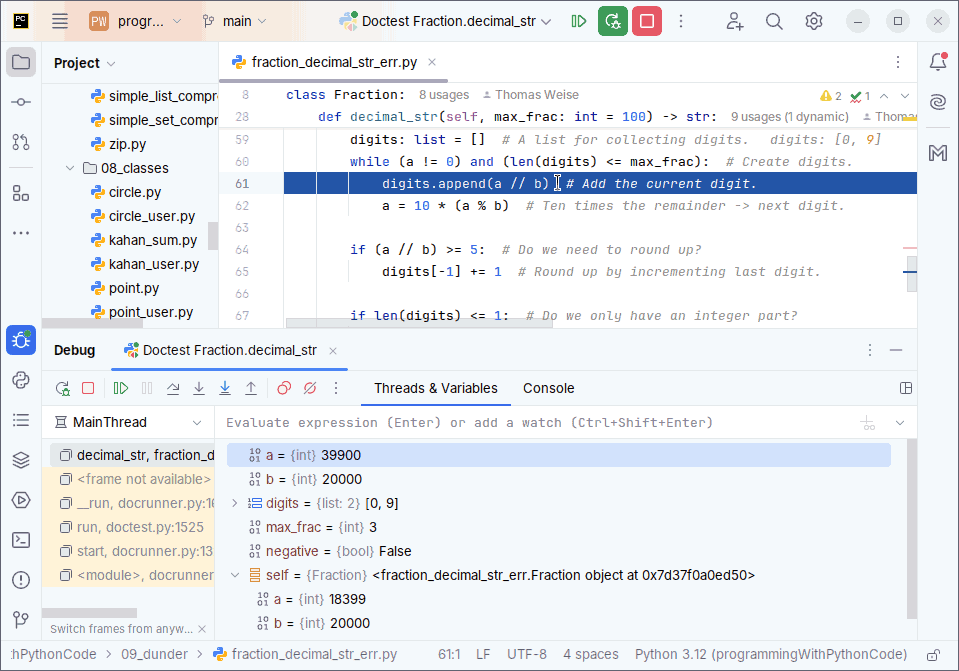
\includegraphics[width=0.48\linewidth]{\currentDir/debug27}}}%
%
\floatSep%
%
\subfloat[][%
\pythonil{1} gets appended to \pythonil{digits}.%
\label{fig:dunder:debug28}%
]{\tightbox{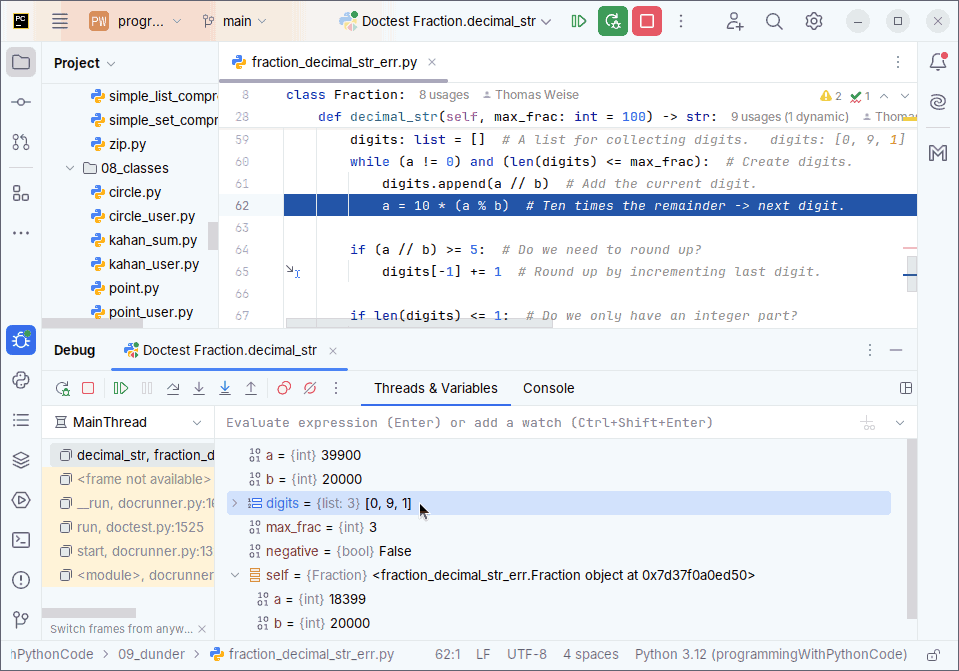
\includegraphics[width=0.48\linewidth]{\currentDir/debug28}}}%
%
\floatRowSep%
%
\subfloat[][%
\pythonil{a} gets updated to \pythonil{199000}.%
\label{fig:dunder:debug29}%
]{\tightbox{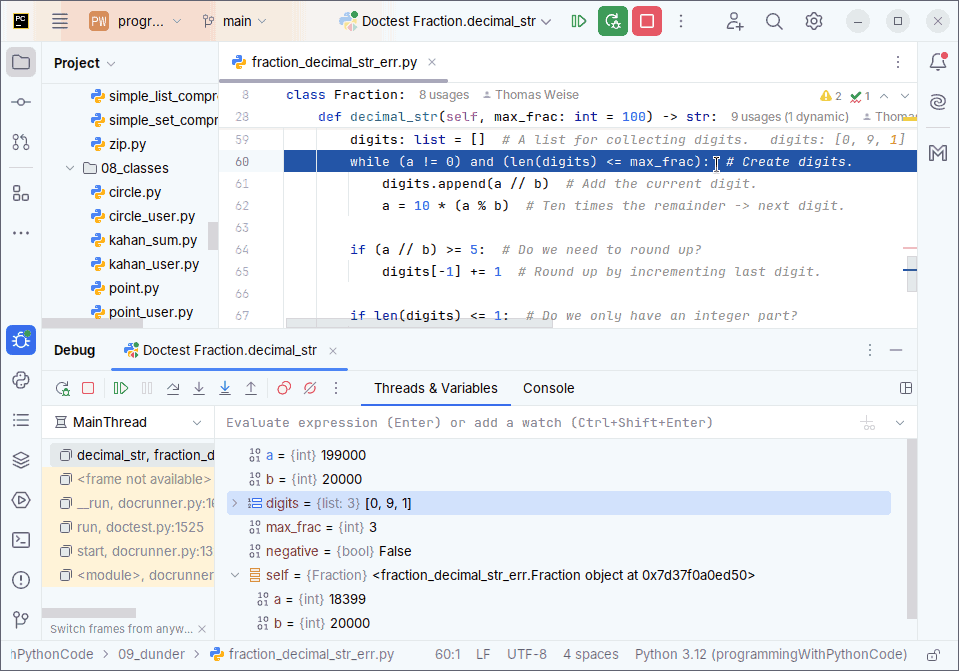
\includegraphics[width=0.48\linewidth]{\currentDir/debug29}}}%
%
\floatSep%
%
\subfloat[][%
The loop condition is still met.%
\label{fig:dunder:debug30}%
]{\tightbox{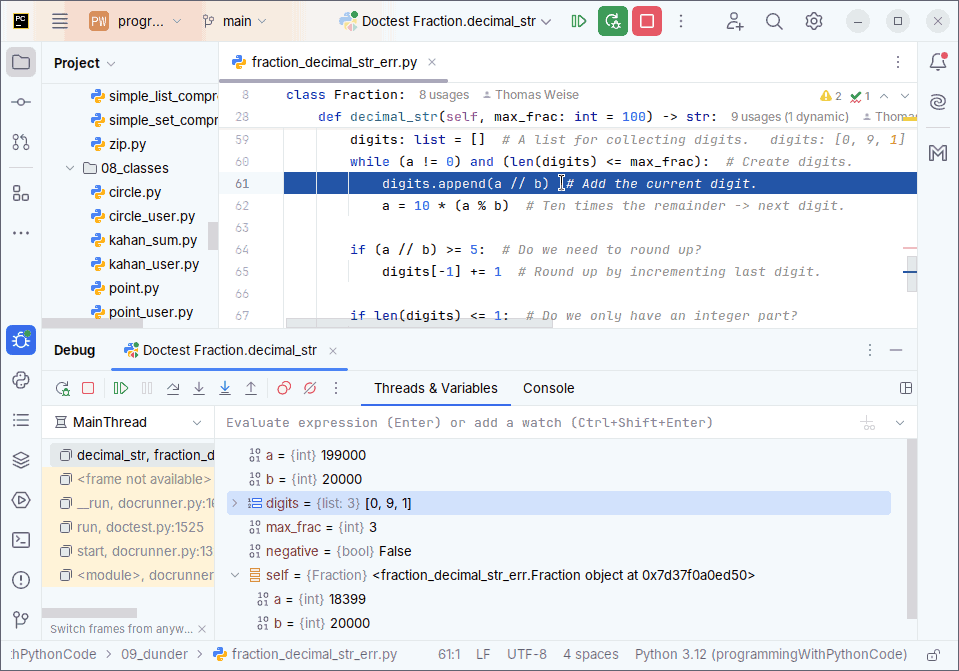
\includegraphics[width=0.48\linewidth]{\currentDir/debug30}}}%
%
%
\caption{Using the \debugger\ in \pycharm~(continued).}%
\label{fig:dunder:debugE}%
\end{figure}%
%
\begin{figure}%
\ContinuedFloat%
\centering%
%
\subfloat[][%
\pythonil{9} gets appended to \pythonil{digits}.%
\label{fig:dunder:debug31}%
]{\tightbox{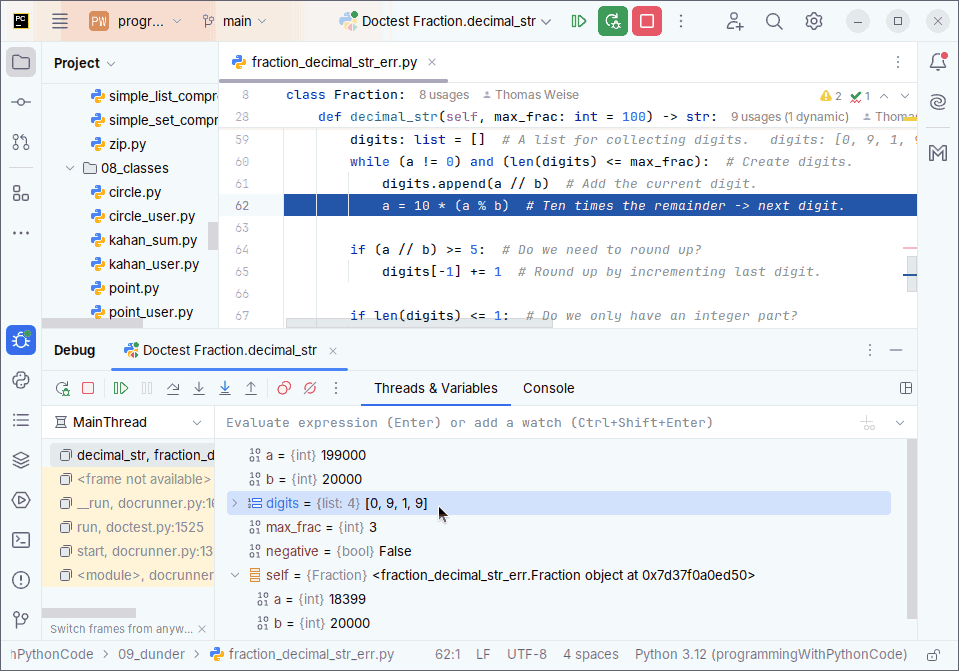
\includegraphics[width=0.48\linewidth]{\currentDir/debug31}}}%
%
\floatSep%
%
\subfloat[][%
\pythonil{a} gets updated to \pythonil{190000}.%
\label{fig:dunder:debug32}%
]{\tightbox{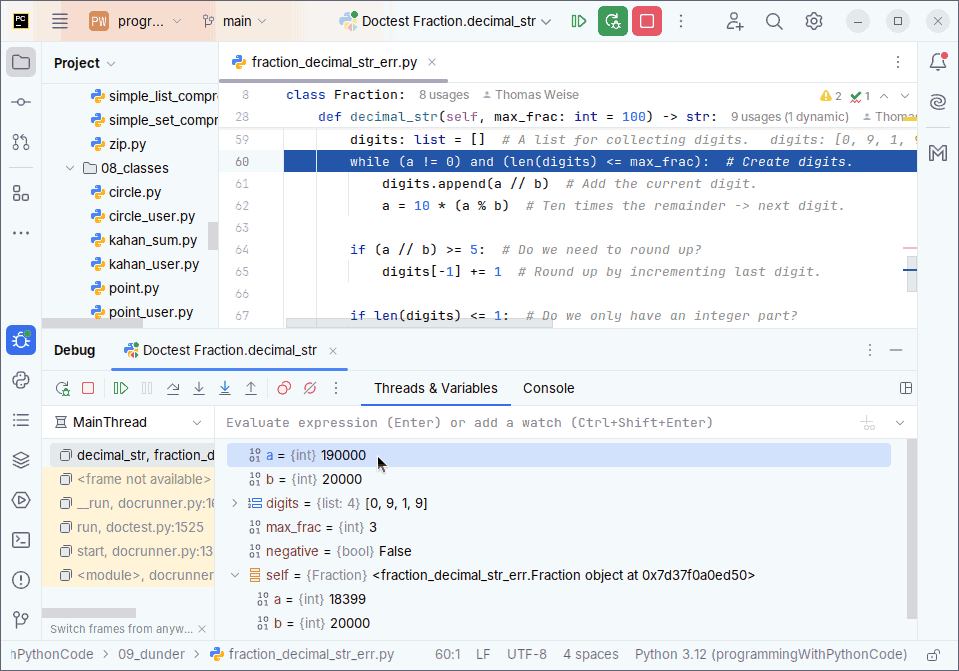
\includegraphics[width=0.48\linewidth]{\currentDir/debug32}}}%
%
\floatRowSep%
%
\subfloat[][%
Since the loop condition evaluates to \pythonil{False}, the cursor is now at the next line after the loop body. %
This line checks whether we should round up the next digit. %
We hit \keys{F8}.%
\label{fig:dunder:debug33}%
]{\tightbox{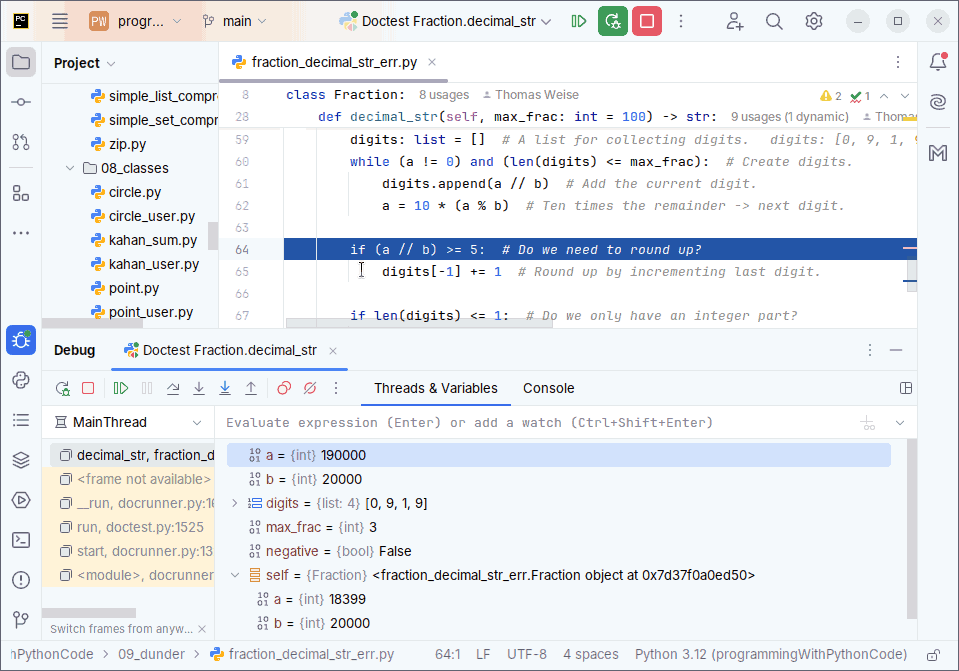
\includegraphics[width=0.48\linewidth]{\currentDir/debug33}}}%
%
\floatSep%
%
\subfloat[][%
The condition of the \pythonil{if} is met, we can now execute its body. %
We press the \pycharmDebuggerStepOver~button.%
\label{fig:dunder:debug34}%
]{\tightbox{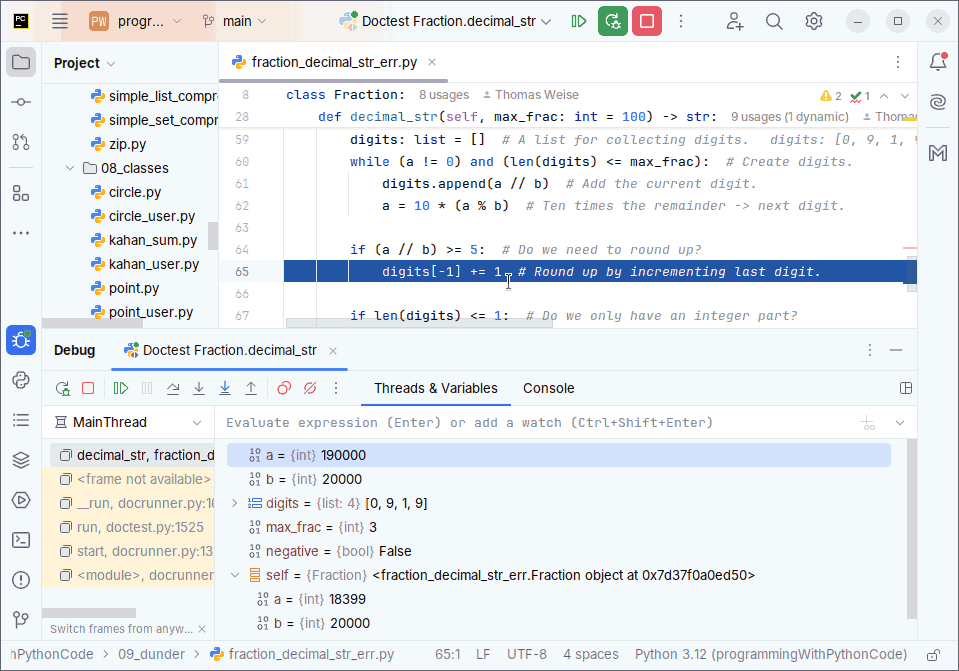
\includegraphics[width=0.48\linewidth]{\currentDir/debug34}}}%
%
\floatRowSep%
%
\subfloat[][%
Our code for rounding up actually turned the last digit into a~\pythonil{10}! %
Because we did not consider that rounding up could cause the next~9 to become a 10, which should be represented as a~0 and lead to the next digit to be rounded up as well.%
\label{fig:dunder:debug35}%
]{\tightbox{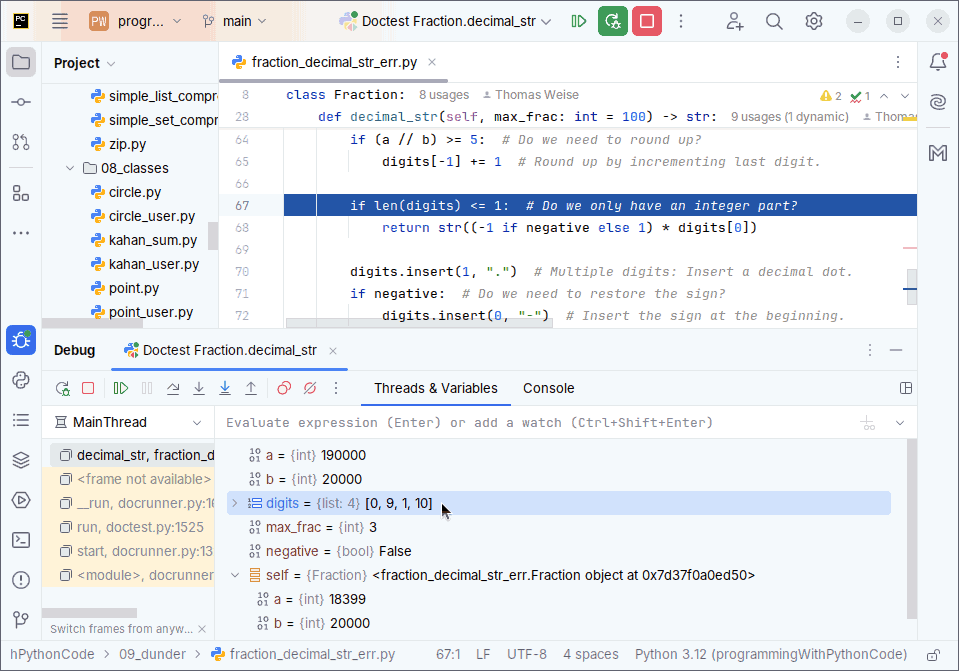
\includegraphics[width=0.8\linewidth]{\currentDir/debug35}}}%
%
\caption{Using the \debugger\ in \pycharm~(continued).}%
\label{fig:dunder:debugF}%
\end{figure}%

In \cref{fig:dunder:debug25,fig:dunder:debug26,fig:dunder:debug27,fig:dunder:debug29,fig:dunder:debug30,fig:dunder:debug31,fig:dunder:debug32} we work our way through the loop in the same way, by pressing \keys{F8} repeatedly.
First, \pythonil{9} gets appended to \pythonil{digits}, then \pythonil{a} gets updated to \pythonil{39900}.
In the following iteration, \pythonil{1} gets appended to \pythonil{digits}, then \pythonil{a} gets updated to \pythonil{199000}.
Then, \pythonil{9} gets appended to \pythonil{digits} and \pythonil{a} gets updated to \pythonil{190000}.

At this stage, \pythonil{digits} has become~\pythonil{[0, 9, 1, 9]}.
Since \pythonil{max_frac} is \pythonil{3}, \pythonil{len(digits) <= max_frac} is no longer~\pythonil{True}.
In \cref{fig:dunder:debug32}, we have arrived back at the head of the loop.
When we hit \keys{F8}, the loop condition is evaluated again, but this time it evaluates to~\pythonil{False}.
The loop terminates and the cursor is placed on the next line of code after the loop.

If we look at what was computed so far, we find that everything is exactly as it should be.
We want to translate the fraction~$\frac{91995}{100000}$ to a decimal string with three fractional digits.
So far, we got the digits~0, 9, 1, and~9.

The next line of code, \pythonil{if (a // b) >= 5}, is supposed to check whether we should round up the last digit.
Since \pythonil{a} is \pythonil{190000} and \pythonil{b} is still \pythonil{20000}, \pythonil{a // b} is~\pythonil{9}.
So the condition should be met.
In \cref{fig:dunder:debug32}, we press the \pycharmDebuggerStepOver~button to find it out.

A look at \cref{fig:dunder:debug35} reveals the bug in our code:
In order to round up, we incremented the last number in our list~\pythonil{digits}.
\pythonil{digits} was~\pythonil{[0, 9, 1, 9]}.
So it is~\pythonil{[0, 9, 1, 10]}.

The strange trailing zeros in our output were not separate digits.
They were the zeros of a ten.
We did not consider that, when rounding up, we do not just have simple cases like~1.25 which we can round to~1.3 by only incrementing one digit.
We can have cases like~0.9999, which rounds up to~1, even if we want three fractional digits of precision.
We can stop the debugging here and go back to our code.%
\clearpage%
%
\gitPython{\programmingWithPythonCodeRepo}{dunder/fraction.py}{--args format --labels part_6}{dunder:fraction:part_6}{%
The repaired Part~6 of the \pythonil{Fraction} class: A correct \pythonil{decimal_str} method.}%

In \cref{lst:dunder:fraction:part_6}, we revisit the \pythonil{decimal_str} method of our class~\pythonil{Fraction}.
Our rounding-up code becomes more complex:
First, we need to loop over all fractional digits, from the end of the list \pythonil{digits} forward:
\pythonil{for i in range(len(digits) - 1, 0, -1)} does this.
If \pythonil{len(digits) == 5}, then \pythonil{range(len(digits) - 1, 0, -1)} iterates over the numbers 4, 3, 2, and~1.
We increment the digit at index~\pythonil{i} by~1.
If it does not become~10, then we can stop the loop via~\pythonilIdx{break}.
If it did become~10, then we set it to zero and continue the loop.
This will increment the next digit, and so on.
If we arrive at index~1 and still need to continue, the regular loop execution ends anyway.

Then, the \pythonil{else} statement is hit.
Recall from \cref{sec:loopElse} that the \pythonil{else}\pythonIdx{for!else} statement at the bottom of a loop is \emph{only} executed if the loop finished regularly, i.e., if no \pythonil{break} statement was executed.
Therefore, if and only if the digit at index~1 also became~10 and was then set to~0, we increment the digit at index~0.
This digit represents the integer part of our fraction.
Here, it is totally OK to round a~9 to a~10.
For example, 9.999 can be rounded to 10, and 1239.9 can be rounded to 1240.

This new code for rounding numbers may introduce zeros at the end of our string.
We just gobble them up with an additional \pythonil{while} loop directly after the rounding.
And with this, we are done.
We have working code converting fractional numbers to decimal strings.
All the \pglspl{doctest} now pass.

\gitPython{\programmingWithPythonCodeRepo}{dunder/fraction_sqrt.py}{--args format}{dunder:fraction_sqrt}{%
Using the \pythonil{Fraction} class to compute square roots.}%
%
\gitOutputTool{\programmingWithPythonCodeRepo}{.}{_scripts_/pytest_doctest.sh dunder fraction_sqrt.py}{dunder:fraction_sqrt:doctest}{%
The (successful) output of \pytest\ executing the \pglspl{doctest} for our \pythonil{sqrt} function from~\cref{lst:dunder:fraction_sqrt} working on instances of the \pythonil{Fraction} class.}

But let's get back to what we actually wanted to do:
We wanted to compute the square roots of numbers at insane precision.
For this, we can now revisit \cref{lst:functions:my_math}.
In \cref{lst:dunder:fraction_sqrt}, we just copy the code of the \pythonil{sqrt} function from this file.
We will basically replace all \pythonils{float} in this code with \pythonils{Fraction}.%
%
\begin{sloppypar}%
The function's signature changes from~\pythonil{def sqrt(number: float) -> float} to \pythonil{def sqrt(number: Fraction) -> Fraction}.
Well, we know that the square roots of some numbers like~$\sqrt{2}$ are irrational, i.e., we cannot represent the exactly with an instance of~\pythonil{Fraction}.
In the original code, due to the limited range of~\pythonils{float}, this is not a problem and the function will eventually stop (when all of the 15 to 16 digits of precision are exhausted).
However, using \pythonil{Fraction}, the same code could loop forever, trying to find better and better approximations.
So we need to limit the iterations with an additional parameter \pythonil{max_steps: int = 10} limiting the number of cycles for our loop.
You will later see that this default value of only permitting ten steps is already quite sufficient to get very nice approximations.%
\end{sloppypar}%
%
In \cref{lst:dunder:fraction_sqrt}, we replace numbers like~\pythonil{0.0}, \pythonil{0.5} and~\pythonil{1.0} with our constants~\pythonil{ZERO}, \pythonil{ONE_HALF}, and~\pythonil{ONE}.
We need to do this because our mathematical dunder methods only work with other instances of~\pythonil{Fraction}.
We could have easily implemented them to also support woring with instances of~\pythonil{int} or~\pythonil{float}, but did not do it (again for the sake of brevity).
Either way, all the numerical constants in \cref{lst:dunder:fraction_sqrt} are now instances of~\pythonil{Fraction}.

Our new function begins with an initial check whether the input number is negative and, if so, raises an~\pythonilIdx{ArithmeticError}.
Then it has basically the same loop and body as our original variant in~\cref{lst:functions:my_math}.
The only difference is that we decrease~\pythonil{max_steps} in each iteration and \pythonil{break} out the loop once it reaches~\pythonil{0}.%
%
\begin{sloppypar}%
We, of course, add \pglspl{doctest} to our function.
For example, we test the expression \pythonil{sqrt(Fraction(2, 1)).decimal_str(750)}.
This computes~$\sqrt{\frac{2}{1}}=\sqrt{2}$ by performing ten steps of Heron's algorithm.
Then it translates to a decimal string with \emph{750 fractional digits}.
We take the correct value from~\cite{S2024DEOSRO2,NB1997TSROTT1MD}.
This means unless our function provides this number of digits correctly \emph{after only ten steps}, the \pgls{doctest} will fail.%
\end{sloppypar}%
%
The second \pgls{doctest} is simply to check whether~$\sqrt{4}$ renders as~2 when converted to a decimal string.
Of course, we just approximate the square root through several steps, so the value of the fraction might not actually be~2.
However, when rendered to 100~digits of precision, it should return~\pythonil{"2"}.

Finally, we want to compute the golden ratio~\numberGoldenRatio~\cite{CEOEB2024GR,EHF2008EEOGTGOJLH11FEEEELIEILHIATBG11EAPWMETBFR,S2024DEOGRPOT}, which equals~$\frac{1+\sqrt{5}}{2}$.
We can write this as \pythonil{ONE_HALF * (ONE + sqrt(Fraction(5, 1)))}.
In the \pgls{doctest}, we want to see whether our results are correct to 420~fractional digits, which we take from~\cite{F1996TGR1T2P}.

The results of the \pglspl{doctest} executed by \pytest\ can be seen in \cref{exec:dunder:fraction_sqrt:doctest}.
They all pass.
All we did was implementing primary school math into a class in \python, together with an algorithm which is almost 2000~years old.
And with \emph{ten steps} of that algorithm, we got approximations of~$\sqrt{2}$ as well as~\numberGoldenRatio\ that were accurate to \emph{several hundreds of digits}.
Isn't that cool?%
%
\FloatBarrier%
\endhsection%
%
\hsection{Implementing Context Managers for the \texttt{with} Statement Revisited}%
\label{sec:dunder:contextManager}%
%
In \cref{sec:withAndContextManagers}, we introduced the \pythonilIdx{with}~block, which is often used to ensure that resources are properly closed after using them.
We used text files as example:
A text file is opened in the head of \pythonilIdx{with} for writing using the \pythonilIdx{open} function.
This function returns a stream to which we then can write strings of text in the body of the \pythonilIdx{with}~block.
Then, after this body ends, the stream is closed automatically.
This happens even if an exception was raised inside the body of the~\pythonilIdx{with}.

Back then, we stated that resources like files are implemented in \python\ as context managers.
A context manager has a special method that is called at the beginning of the \pythonilIdx{with}~block.
The method can be used to \inQuotes{open} the resource, for example.
The context manager also has a special method that is called at the end the \pythonilIdx{with}~block.
This special method can be used to \inQuotes{close} the resource.

At this stage, it will not surprise you that these \inQuotes{special methods} are actually dunder methods.
These methods are \pythonilIdx{\_\_enter\_\_} and \pythonilIdx{\_\_exit\_\_}.
Since \pythonilIdx{with}~blocks are nice syntactical sugar of the \python\ language, we will here play around with them a little bit.

As example, let us create a simple API that allows us to write output in a subset of the \glsreset{XML}\pgls{XML} format~\cite{BPSMM2008EMLX1FE,K2019ITXJY,CH2013XFCAMLTMC}.
\pgls{XML} is a format for data interchange which was predominant in distributed systems the~2000s.
After that, it began to fade out in favor~\cite{A2020XLATDOEOL} of \pgls{JSON}~\cite{E2017SE4TJDIS,RFC8259} and \pgls{YAML}~\cite{DNMAASBE2021YAMLYV1,K2019ITXJY,CGTYB2022YFFDCAIE}.
It is still very relevant today, for example, as foundation of several document formats such as those used in \libreoffice~\cite{DF2024LTDF,GL2012LTSOOSSCBAFACSOL} and \microsoftWord~\cite{MS2024MW,DR2019STFAWAUMW}, or as the basis for the \pgls{SVG} format~\cite{DDGLMSWFJJ2011SVGSSE}.
If you are a bit familiar with web design, then you will find that \pgls{XML} looks a bit like \pgls{HTML}~\cite{HBFLDNOP2014HAVAAAFHAX}.%
%
\begin{sloppypar}%
As shown below, an \pgls{XML}~documents begins with the \pgls{XML} version declaration~\xmlil{<?xml version="1.0"?>}.
Then, it includes \pgls{XML}~elements that can be arbitrarily nested.
Each elements has a name and begins with an opening and closing string, looking somewhat like~\xmlil{<name>...</name>}.
Between the opening and closing string, text and other elements can be included.
An element can have attributes stored in the opening string, which looks like~\xmlil{<name key='value'... >...}.%
\end{sloppypar}%
%
\begin{center}
\begin{minipage}{\linewidth}%
\begin{lstlisting}[style=xml_style]
<?xml version="1.0"?>
<class title='Programming with Python' year='2024'>
    <description>This is a class on Python.</description>
    <teacher name='Thomas'>I like Python.</teacher>
    <students>
        <student name='Bubba'></student>
        <student name='Bibba'>I like the &#38;Programming with Python&#62; book.</student>
    </students>
</class>
\end{lstlisting}%
\end{minipage}%
\end{center}%
%
Here we have a nicely formatted \pgls{XML} text about this course.
The \xmlil{<class>} element has two attributes, \xmlil{title} and \xmlil{year}.
It contains other elements, such as \xmlil{<description>} with a brief description of the class.
Then follows the element \xmlil{<teacher>} with an attribute storing my given name as well as brief text.
Finally, there is an element \xmlil{<students>}, which, in turn, holds two elements of type \xmlil{<student>}.
Each of them hold the student's given name as attribute \xmlil{name}.
The second \xmlil{<student>} element includes some additional text.
In this next, you notice that two characters have been \emph{escaped}: since \textil{<} and \textil{>} are used to mark the beginning and ending of the start and end element strings, they should not occur inside the normal text, as this may confuse the \pgls{XML} parsers.
Therefore, they are escaped as entities~\xmlil{&#38;} and~\xmlil{&#62;}.

\gitPython{\programmingWithPythonCodeRepo}{dunder/xml_context.py}{--args format --labels part_1}{dunder:xml_context:part_1}{%
Part~1 of our very simply context manager-based \pgls{XML} output API.}%
%
\gitPython{\programmingWithPythonCodeRepo}{dunder/xml_context.py}{--args format --labels part_2}{dunder:xml_context:part_2}{%
Part~2 of our very simply context manager-based \pgls{XML} output API.}%

Would it not be nice to have a simple \pgls{API} that allows us to produce valid~\pgls{XML} and that takes care of the escaping of special characters?
While countless such tools already exist {\dots} let us make our own.
For this, we realize:
First, every \pgls{XML} element that is opened must also be closed.
Second, \pgls{XML} elements can be nested arbitrarily.
This kind of looks like an application of the \pythonilIdx{with} statement.

We now make our own context manager.
When the \pythonilIdx{with} statement begins, our context manager will write the element start text.
Inside the body of the \pythonilIdx{with}~statement, we will allow to write the element text or to open sub-elements.
At the end of the \pythonilIdx{with}~statement, the \pgls{XML} element closing text should be written.
Furthermore, we want to be able to direct the output of our \pgls{API} to any destination where strings can be written to, say, \pythonil{print}, to \pythonils{list}, or to files.
As you will see in \cref{lst:dunder:xml_context:part_1,lst:dunder:xml_context:part_2}, we can implement all of that in a fairly small module.

In \cref{lst:dunder:xml_context:part_1}, we begin by defining an internal constant \pythonil{_ESC}, which we use for \pgls{XML} escaping special characters in strings with \pgls{XML}~entities.
For this purpose, we use the functions \pythonilIdx{maketrans}\pythonIdx{str!maketrans} and \pythonilIdx{translate}\pythonIdx{str!translate} of the class~\pythonilIdx{str}.
The former accepts a dictionary where the keys are single characters and the corresponding values are strings with which these characters should be replaced.
It creates some \python-internal datastructure which then can be passed to \pythonilIdx{translate}\pythonIdx{str!translate} to perform the replacement.
For example, we could do~\pythonil{x = str.maketrans(\{"A": "XYZ"\})}.
Then, \pythonil{"ABCBA".translate(x)} would yield~\pythonil{"XYZBCBXYZ"}.
This is very useful to painlessly implement rudimentary support to escape special characters based on the \pgls{XML}~standard~\cite{BPSMM2008EMLX1FE}.

Then we define the \pythonil{class Element}.
The initializer~\dunder{init} of this class has four important parameters.
\pythonil{dest}~is a \pythonilIdx{Callable}, i.e., function, that can accept a single string as parameter.
This will be where all the output of our API is sent to.
\pythonil{name}~is a string with the name of the element.
\pythonil{attrs}~contains the attributes of the element.
It is either \pythonil{None} if there are no attributes (which is the default).
Otherwise, it is a \pythonilIdx{dict} mapping string keys to arbitrary values.
Finally, \pythonil{is_root} is a Boolean value that is \pythonil{True} if this element is the single root element of the \pgls{XML}~document that we want to write, and \pythonil{False} if it is some nested element.
This is needed, because before writing the root element, the \pgls{XML} version declaration~\xmlil{<?xml version="1.0"?>} must be written.
This must happen only once and only at the beginning of an \pgls{XML}~document.

In the initializer, we store the \pythonil{dest} argument in an attribute that is both private~(signified by the two leading underscores) and immutable~(signified by the \pgls{typeHint}~\pythonilIdx{Final}).
We then construct the element start string by filling a list~\pythonil{head} and store its concatenated elements in the attribute~\pythonil{__head}.
Only if our element is a root element, the \pgls{XML} version declaration is included in the list~\pythonil{head}.
The actual element start string begins by the less-than symbol and the element name~(\xmlil{<name}).
Then, if \pythonil{attrs} is neither \pythonil{None} nor empty, we want to add the attributes.
Interestingly, this condition can be expressed by a simple~\pythonil{if attrs:}.
If there are attributes, then we iterate over the key-value pairs in~\pythonil{attrs} by writing~\pythonil{for key, value in attrs.items():}.
We use an~\pgls{fstring} composed of the \pythonil{key} and a string for the value, which we construct in a clever way:
Since we permit arbitrary value types, we convert the \pythonil{value} to a string first, using the \pythonilIdx{str}~function.
Then, we escape special characters, using the aforementioned \pythonilIdx{translate}\pythonIdx{str!translate} routine with our map~\pythonil{_ESC}.
It should be noted that only character here that needs to actually be escaped is the \inQuotes{\textil{'}}~character, which therefore also was included in the construction of~\pythonil{_ESC}.
This is because we also use this character to delimit our strings:
The \pythonil{!r} format specifier in the \pgls{fstring} adds these single quotation marks.
Finally, the element start string ends with~\pythonil{">"}.
With \pythonil{"".join(head)}\pythonIdx{join}\pythonIdx{str!join}, all strings in the list~\pythonil{head} are merged into one.%
%
\begin{sloppypar}%
Constructing the element end string is much easier, we simply write~\pythonil{self.__foot: Final[str] = f"</{name}>"}.
Notice that, so far, we have just cached strings and did not yet write anything to the output~\pythonil{dest}.%
\end{sloppypar}%
%
\begin{sloppypar}%
This should come when a \pythonilIdx{with} body begins.
At this moment, the \python~interpreter will call the method \pythonilIdx{\_\_enter\_\_}\pythonIdx{dunder!\_\_enter\_\_} of the context manager.
All we need to do in this method is to invoke~\pythonil{self.__dest(self.__head)}.
If \pythonil{__dest} was, for example, the \pythonil{print}~function, this would write the element start to the \pgls{stdout}.
The method \pythonilIdx{\_\_enter\_\_}\pythonIdx{dunder!\_\_enter\_\_} also must return an object which can be assigned to a variable for use inside the \pythonilIdx{with} block using the \pythonilIdx{as} statement.
We here want to return our \pythonil{Element} object itself, so we write~\pythonil{return self}.
The proper \pgls{typeHint} for the return type in such situations is~\pythonilIdx{Self}\pythonIdx{typing!Self}.%
\end{sloppypar}%
%
\bestPractice{typeHintSelf}{%
Methods that return~\pythonilIdx{self} should be annotated with the \pgls{typeHint}~\pythonilIdx{Self}\pythonIdx{typing!Self}~\cite{PEP673}. %
Static code analysis tools then see that the method always returns an object of the same class as the object itself.%
}%
%
Either way, \pythonilIdx{\_\_enter\_\_}\pythonIdx{dunder!\_\_enter\_\_} will be called at the beginning of a \pythonilIdx{with} statement.
At the end of an \pythonilIdx{with} statement, in other words, when we are done using our object, the \pythonilIdx{\_\_exit\_\_}\pythonIdx{dunder!\_\_exit\_\_} method will be called.
Then, we should write the element end text stored in the attribute~\pythonil{__foot}.
Therefore, we write \pythonil{self.__dest(self.__foot)}.

The \pythonilIdx{\_\_exit\_\_}\pythonIdx{dunder!\_\_exit\_\_} method looks a bit different from \pythonilIdx{\_\_enter\_\_}\pythonIdx{dunder!\_\_enter\_\_}.
First, it also gets three parameters: the exception type~\pythonil{exc_type}, the exception value~\pythonil{exc_value}, and the stack~\pythonil{traceback}.
These parameters are filled with the information about any \pythonilIdx{Exception} raised within the \pythonilIdx{with}~body.
Otherwise, they will be~\pythonil{None}~\cite{PSF2024WSCM}.
We here just define a single parameter~\pythonil{*exc}.
This syntax tells \python\ to capture all positional arguments into a single tuple.
Since we do not care about exceptions here, we just write this to safe space, honestly, because I do not want to write three lines of \pgls{docstring} where one suffices.
All we want is to write the element end string.
We then always return~\pythonil{False}, which basically tells the \python~interpreter:
\emph{\inQuotes{If any exception occurred inside the \pythonilIdx{with} statement, please raise this exception again after we are finished with~\pythonilIdx{\_\_exit\_\_}\pythonIdx{dunder!\_\_exit\_\_}.}}
The proper \pgls{typeHint} for this is \pythonil{Literal[False]}\pythonIdx{Literal}\pythonIdx{typing!Literal}.%
%
\bestPractice{returnLiteralTypeHint}{%
If a parameter of a function can take on only some special constant values~\pythonil{X}, say certain integers or strings, the proper \pgls{typeHint} is \pythonil{Literal[X]}\pythonIdx{Literal}\pythonIdx{typing!Literal}~\cite{PEP586}. %
The same holds if your function always returns the same, simple constant(s)~\pythonil{X}.%
}%
%
With this, we have basically completed implementing our context manager.
What is still missing is some functionality to write text into an element and to convenient branching off new sub-elements.

The former is very easy:
We define a method~\pythonil{text} taking a string~\pythonil{txt} as input parameter.
All we have to do in the body of this method is~\pythonil{self.__dest(txt.translate(_ESC))}.
This escapes any dangerous \pgls{XML} special characters in the string and passes the result on to the output destination.

The method~\pythonil{element} is used to branch off new sub-elements.
It basically would take the same parameters as the initializer~\pythonil{\_\_init\_\_}.
However, the new element must use the same output destination and it cannot be a root element (because it is a sub-element).
Therefore, we only need to pass the parameters~\pythonil{name} and~\pythonil{attrs} to a new instance of~\pythonil{Element}, whereas we hand over \pythonil{self.__dest} as destination and \pythonil{False} as \pythonil{is_root}.
With this, our simple \pgls{API} for a subset of the \pgls{XML} standard~\cite{BPSMM2008EMLX1FE} is already completed.%
%
\gitPythonAndOutputFormat{xml_style}%
\gitPythonAndOutput{\programmingWithPythonCodeRepo}{dunder}{xml_user_print.py}{--args format}{dunder:xml_user_print}{%
An example of using our simple context manager-based \pgls{XML} output API from \cref{lst:dunder:xml_context:part_1,lst:dunder:xml_context:part_2}, where the output is printed to the \pgls{stdout}.}%
%
\gitPythonAndOutputFormat{xml_style}%
\gitPythonAndOutput{\programmingWithPythonCodeRepo}{dunder}{xml_user_file.py}{--args format}{dunder:xml_user_file}{%
An example of using our simple context manager-based \pgls{XML} output API from \cref{lst:dunder:xml_context:part_1,lst:dunder:xml_context:part_2}, where the output is written to a text file\pythonIdx{write}\pythonIdx{IO!write}\pythonIdx{open}\pythonIdx{remove}\pythonIdx{os!remove}.}%

We now use this \pgls{API} in \cref{lst:dunder:xml_user_print,lst:dunder:xml_user_file} to basically reproduce the small \pgls{XML}~snippet that I showed you before.
In the former example, we use \pythonil{print} as destination function.
This means that any string that our \pgls{API} passes to its internal \pythonil{__dest}~attribute will immediately be written as a single line to the~\pgls{stdout}.

We begin by creating the \xmlil{<class>} element with the \xmlil{title} and \xmlil{year} attributes.
We do this by creating a new instance of~\pythonil{Element} in a \pythonilIdx{with} block and by passing on the attributes as~\pythonil{dict}.
This object is stored as variable~\pythonil{cls} via the \inQuotes{\pythonilIdx{as}}~statement.
We the create the \xmlil{description} element by writing \pythonil{with cls.element("description") as desc}.
The class description can then be written via \pythonil{desc.text(...)}.
Notice that our \pgls{API} writes the element start and end strings to the output without requiring us to do anything.
It also escapes all special characters for us.
The other elements are created in the same convenient fashion.
Our \python\ code basically mirrors the \pgls{XML} structure.
The output of the program in \cref{exec:dunder:xml_user_print} looks very much like our example, with a slightly different indentation and line breaking.
But this is permitted and acceptable under the \pgls{XML} standard~\cite{BPSMM2008EMLX1FE}.

Instead of writing to the \pgls{stdout}, we can also recall our very first example for the \pythonilIdx{with} statement back in \cref{sec:withAndContextManagers}:
writing to and reading from a file.
\Cref{lst:dunder:xml_user_file} is almost exactly the same as \cref{lst:dunder:xml_user_print}.
The difference is that we now \pythonilIdx{open} a text output stream~\pythonil{stream_out} to a file~\textil{example.xml} and the stream's~\pythonilIdx{write}\pythonIdx{IO!write}~method as destination to our~\pgls{API}.
As a result, all the text is now written to a file instead.

We later \pythonilIdx{open} the file again and read all of its lines one-by-one via the~\pythonil{for line in stream_in} loop.
Files are actually \pythonilsIdx{Iterator} of line strings!
All the file contents get written to the \pgls{stdout}.
Since \pythonilIdx{write} does not append newline characters, this format is much more compact, as can be seen in~\cref{exec:dunder:xml_user_file}.
But it is perfectly valid~\pgls{XML}.

We now have learned how the functionality of the \pythonilIdx{with}~statement is implemented internally.
And we used it to hammer together a very compact and yet functional \pgls{API} for a subset of the \pgls{XML} standard~\cite{BPSMM2008EMLX1FE}.
Obviously, we do not implement the complete standard, which is much more complicated.
And you should never use our class if you really wanted to produce \pgls{XML} in a productive code.
We also omitted type and sanity checks -- for example, we should forbid element names that are empty or contain special characters like~\textil{<}.
A real implementation would be more conservative~(and too long to serve as a good example in this book).
Still, on one hand, our \pgls{XML} is valid.
On the other hand, you \emph{could} use extend and improve this class to have all the functionality that you need, if you wanted to.
So this is actually another example that, at this stage and with what you have learned, you can already do real things.%
%
\FloatBarrier%
\endhsection%
%
\hsection{Overview over Dunder Methods}%
%
\begin{figure}%
\renewcommand*\DTstylecomment{\relax}%
\renewcommand*\DTstyle{\small}%
%
\dirtree{%
.1 \pythonilIdx{\_\_}.
.2 String Representation, see \cref{sec:strReprEq}.
.3 \dunder{str}\DTcomment{returns a concise string representation for users; \pythonil{str(a)}\pythonIdx{str}~$\cong$~\pythonil{a.\_\_str\_\_()}}.
.3 \dunder{repr}\DTcomment{string with all information on the object for programmers; \pythonil{repr(a)}\pythonIdx{repr}~$\cong$~\pythonil{a.\_\_repr\_\_()}}.
.3 \dunder{format}\DTcomment{used in \pglspl{fstring}: \pythonil{f"\{a:s\}"}~$\cong$~\pythonil{a.\_\_format\_\_(s)}}.
.2 Type Conversion.
.3 \dunder{bool}\DTcomment{convert to \pythonilIdx{bool}: \pythonil{bool(a)}\pythonIdx{bool}~$\cong$~\pythonil{a.\_\_bool\_\_()}; used in conditions, e.g, in~\pythonil{if}}.
.3 \dunder{int}\DTcomment{convert to \pythonilIdx{int}: \pythonil{int(a)}\pythonIdx{int}~$\cong$~\pythonil{a.\_\_int\_\_()}}.
.3 \dunder{float}\DTcomment{convert to \pythonilIdx{float}: \pythonil{float(a)}\pythonIdx{float}~$\cong$~\pythonil{a.\_\_float\_\_()}}.
.3 \dunder{complex}\DTcomment{convert to \pythonilIdx{complex}: \pythonil{complex(a)}~$\cong$~\pythonil{a.\_\_complex\_\_()}}.
.3 \dunder{bytes}\DTcomment{convert to \pythonilIdx{bytes}: \pythonil{bytes(a)}~$\cong$~\pythonil{a.\_\_bytes\_\_()}}.
.2 Hashing, see \cref{sec:hashDunder}.
.3 \dunder{hash}\DTcomment{compute an integer value representing this object; \pythonil{hash(a)}~$\cong$~\pythonil{a.\_\_hash\_\_()}}.
.2 Ordering and Equality, see \cref{sec:arithmeticsAndOrder}.
.3 \dunder{eq}\DTcomment{equality: \pythonil{a == b}\pythonIdx{==}~$\cong$~\pythonil{a.\_\_eq\_\_(b)}}.
.3 \dunder{ne}\DTcomment{inequality: \pythonil{a != b}\pythonIdx{"!==}~$\cong$~\pythonil{a.\_\_ne\_\_(b)}}.
.3 \dunder{lt}\DTcomment{less than: \pythonil{a < b}\pythonIdx{<}~$\cong$~\pythonil{a.\_\_lt\_\_(b)}}.
.3 \dunder{le}\DTcomment{less than or equal: \pythonil{a <= b}\pythonIdx{<=}~$\cong$~\pythonil{a.\_\_le\_\_(b)}}.
.3 \dunder{gt}\DTcomment{greater than: \pythonil{a > b}\pythonIdx{>}~$\cong$~\pythonil{a.\_\_gt\_\_(b)}}.
.3 \dunder{ge}\DTcomment{greater than or equal: \pythonil{a >= b}\pythonIdx{>=}~$\cong$~\pythonil{a.\_\_ge\_\_(b)}}.
.2 Context Managers, see \cref{sec:dunder:contextManager}.
.3 \dunder{enter}\DTcomment{enter a \pythonil{with a as x}\pythonIdx{with} statement, returns the value~\pythonil{x} given to \pythonilIdx{as}}.
.3 \dunder{exit}\DTcomment{leave a \pythonilIdx{with} statement, receive exception information, returns~\pythonil{False} to re-raise caught exceptions, if any}.
.2 Collections.
.3 \dunder{len}\DTcomment{get the number of elements in container; \pythonil{len(a)}\pythonIdx{len}~$\cong$~\pythonil{a.\_\_len\_\_()}}.
.3 \dunder{contains}\DTcomment{check whether element is present; \pythonil{x in a}\pythonIdx{in}~$\cong$~\pythonil{a.\_\_contains\_\_(x)}}.
.3 \dunder{getitem}\DTcomment{get element at index/key; \pythonil{a[x]}~$\cong$~\pythonil{a.\_\_getitem\_\_(x)}}.
.3 \dunder{setitem}\DTcomment{set element at index/key; \pythonil{a[x]=y}~$\cong$~\pythonil{a.\_\_setitem\_\_(x, y)}}.
.3 \dunder{delitem}\DTcomment{delete element at index/key; \pythonil{del a[x]}\pythonIdx{del}~$\cong$~\pythonil{a.\_\_detitem\_\_(x)}}.
.2 Iteration, see \cref{sec:iterable}.
.3 \dunder{iter}\DTcomment{get iterator over elements; \pythonil{iter(a)}\pythonIdx{iter}~$\cong$~\pythonil{a.\_\_iter\_\_()}}.
.3 \dunder{next}\DTcomment{get next element from iterator; \pythonil{next(i)}~$\cong$~\pythonil{i.\_\_next\_\_()}}.
.3 \dunder{reversed}\DTcomment{iterate backwards; \pythonil{reverse(a)}~$\cong$~\pythonil{a.\_\_reversed\_\_()}}.
.2 Classes.
.3 \dunder{new}\DTcomment{create a new instance of a class: \pythonil{cls(a, b=c)}~$\cong$~\pythonil{cls.\_\_new\_\_(cls, a, b=c)}, is then followed by~\pythonil{cls.\_\_init\_\_(a, b=c)}}.
.3 \dunder{init}\DTcomment{initialize an object: \pythonil{cls(a, b=c)}~$\cong$~\pythonil{cls.\_\_init\_\_(a, b=c)}}.
.3 \dunder{call}\DTcomment{call an object like a function: \pythonil{a(b, c=d)}~$\cong$~\pythonil{a.\_\_call\_\_(b, c=d)}}.
}%
%
\caption{An overview of the dunder\pythonIdx{dunder} methods in \python\ (Part~1).}%
\label{fig:pythonDunder:1}%
\end{figure}%
%
\begin{figure}%
\renewcommand*\DTstylecomment{\relax}%
\renewcommand*\DTstyle{\small}%
%
\dirtree{%
.1 \pythonilIdx{\_\_}.
.2 Arithmetics, see \cref{sec:arithmeticsAndOrder} for selected examples.
.3 \dunder{abs}\DTcomment{absolute value: \pythonil{abs(a)}\pythonIdx{abs}~$\cong$~\pythonil{a.\_\_abs\_\_()}}.
.3 \dunder{minus}\DTcomment{negate: \pythonil{-a}\pythonIdx{-}~$\cong$~\pythonil{a.\_\_minus\_\_()}}.
.3 \dunder{pos}\DTcomment{positive: \pythonil{+a}\pythonIdx{+}~$\cong$~\pythonil{a.\_\_pos\_\_()}}.
.3 \dunder{invert}\DTcomment{invert: \pythonil{\~a}\pythonIdx{\texttildelow}~$\cong$~\pythonil{a.\_\_invert\_\_()}}.
.3 \dunder{add}\DTcomment{add: \pythonil{a + b}\pythonIdx{+}~$\cong$~\pythonil{a.\_\_add\_\_(b)}}.
.3 \dunder{radd}\DTcomment{right-add: \pythonil{a + b}\pythonIdx{+}~$\cong$~\pythonil{b.\_\_radd\_\_(a)}, if \pythonil{a.\_\_add\_\_(b)} yields~\pythonilIdx{NotImplemented}}.
.3 \dunder{sub}\DTcomment{subtract: \pythonil{a - b}\pythonIdx{-}~$\cong$~\pythonil{a.\_\_sub\_\_(b)}}.
.3 \dunder{rsub}\DTcomment{right-subtract: \pythonil{a - b}\pythonIdx{-}~$\cong$~\pythonil{b.\_\_rsub\_\_(a)}, if \pythonil{a.\_\_sub\_\_(b)} yields~\pythonilIdx{NotImplemented}}.
.3 \dunder{mul}\DTcomment{multiply: \pythonil{a * b}\pythonIdx{*}~$\cong$~\pythonil{a.\_\_mul\_\_(b)}}.
.3 \dunder{rmul}\DTcomment{right-multiply: \pythonil{a * b}\pythonIdx{*}~$\cong$~\pythonil{b.\_\_rmul\_\_(a)}, if \pythonil{a.\_\_mul\_\_(b)} yields~\pythonilIdx{NotImplemented}}.
.3 \dunder{truediv}\DTcomment{divide: \pythonil{a / b}\pythonIdx{/}~$\cong$~\pythonil{a.\_\_truediv\_\_(b)}}.
.3 \dunder{rtruediv}\DTcomment{right-divide: \pythonil{a / b}\pythonIdx{/}~$\cong$~\pythonil{b.\_\_rtruediv\_\_(a)}, if \pythonil{a.\_\_truediv\_\_(b)} yields~\pythonilIdx{NotImplemented}}.
.3 \dunder{mod}\DTcomment{modulo-divide: \pythonil{a \% b}\pythonIdx{\%}~$\cong$~\pythonil{a.\_\_mod\_\_(b)}}.
.3 \dunder{rmod}\DTcomment{right-modulo-divide: \pythonil{a \% b}\pythonIdx{\%}~$\cong$~\pythonil{b.\_\_rmod\_\_(a)}, if \pythonil{a.\_\_mod\_\_(b)} yields~\pythonilIdx{NotImplemented}}.
.3 \dunder{floordiv}\DTcomment{integer-divide: \pythonil{a // b}\pythonIdx{//}~$\cong$~\pythonil{a.\_\_floordiv\_\_(b)}}.
.3 \dunder{rfloordiv}\DTcomment{right-integer-divide: \pythonil{a // b}\pythonIdx{//}~$\cong$~\pythonil{b.\_\_rfloordiv\_\_(a)}, if \pythonil{a.\_\_floordiv\_\_(b)} yields~\pythonilIdx{NotImplemented}}.
.3 \dunder{pow}\DTcomment{exponential: \pythonil{a ** b}\pythonIdx{**}~$\cong$~\pythonil{a.\_\_pow\_\_(b)}}.
.3 \dunder{rpow}\DTcomment{right-exponential: \pythonil{a ** b}\pythonIdx{**}~$\cong$~\pythonil{b.\_\_rpow\_\_(a)}, if \pythonil{a.\_\_pow\_\_(b)} yields~\pythonilIdx{NotImplemented}}.
.3 \dunder{matmul}\DTcomment{matrix-multiply: \pythonil{a @ b}\pythonIdx{@}~$\cong$~\pythonil{a.\_\_matmul\_\_(b)}}.
.3 \dunder{rmatmul}\DTcomment{right-ma, see \cref{sec:arithmeticsAndOrder}trix-multiply: \pythonil{a @ b}\pythonIdx{@}~$\cong$~\pythonil{b.\_\_rmatmul\_\_(a)}, if \pythonil{a.\_\_matmul\_\_(b)} yields~\pythonilIdx{NotImplemented}}.
.3 \dunder{divmod}\DTcomment{compute the result of an integer division as well as the remainder and return them as 2-tuple: \pythonil{divmod(a, b)}\pythonIdx{divmod}~$\cong$~\pythonil{a.\_\_divmod\_\_(b)}}.
.3 \dunder{rdivmod}\DTcomment{right-sided \pythonilIdx{divmod}: \pythonil{divmod(a, b)}\pythonIdx{divmod}~$\cong$~\pythonil{b.\_\_divmod\_\_(a)}, if \pythonil{a.\_\_divmod\_\_(b)} yields~\pythonilIdx{NotImplemented}}.
.3 \dunder{round}\DTcomment{round: \pythonil{round(a)}\pythonIdx{round}~$\cong$~\pythonil{a.\_\_round\_\_()}}.
.3 \dunder{trunc}\DTcomment{truncated to integer: \pythonil{math.trunc(a)}\pythonIdx{trunc}\pythonIdx{math!trunc}~$\cong$~\pythonil{a.\_\_trunc\_\_()}}.
.3 \dunder{floor}\DTcomment{round towards~$-\infty$: \pythonil{math.floor(a)}\pythonIdx{floor}\pythonIdx{math!floor}~$\cong$~\pythonil{a.\_\_floor\_\_()}}.
.3 \dunder{ceil}\DTcomment{round towards~$+\infty$: \pythonil{math.ceil(a)}\pythonIdx{ceil}\pythonIdx{math!ceil}~$\cong$~\pythonil{a.\_\_ceil\_\_()}}.
.2 In-Place Arithmetics.
.3 \dunder{iadd}\DTcomment{in-place addition: \pythonil{a += b}\pythonIdx{+=}~$\cong$~\pythonil{a.\_\_iadd\_\_(b)}, returns~\pythonilIdx{self}}.
.3 \dunder{isub}\DTcomment{in-place subtraction: \pythonil{a -= b}\pythonIdx{-=}~$\cong$~\pythonil{a.\_\_isub\_\_(b)}, returns~\pythonilIdx{self}}.
.3 \dunder{imul}\DTcomment{in-place multiplication: \pythonil{a *= b}\pythonIdx{*=}~$\cong$~\pythonil{a.\_\_imul\_\_(b)}, returns~\pythonilIdx{self}}.
.3 \dunder{itruediv}\DTcomment{in-place division: \pythonil{a /= b}\pythonIdx{/=}~$\cong$~\pythonil{a.\_\_itruediv\_\_(b)}, returns~\pythonilIdx{self}}.
.3 \dunder{imod}\DTcomment{in-place modulo division: \pythonil{a \%= b}\pythonIdx{\%=}~$\cong$~\pythonil{a.\_\_imod\_\_(b)}, returns~\pythonilIdx{self}}.
.3 \dunder{ifloordiv}\DTcomment{in-place integer division: \pythonil{a //= b}\pythonIdx{//=}~$\cong$~\pythonil{a.\_\_ifloordiv\_\_(b)}, returns~\pythonilIdx{self}}.
.3 \dunder{ipow}\DTcomment{in-place exponentiation: \pythonil{a **= b}\pythonIdx{**=}~$\cong$~\pythonil{a.\_\_ipow\_\_(b)}, returns~\pythonilIdx{self}}.
.3 \dunder{imatmul}\DTcomment{in-place matrix multiplication: \pythonil{a @= b}\pythonIdx{@=}~$\cong$~\pythonil{a.\_\_imatmul\_\_(b)}, returns~\pythonilIdx{self}}.
}%
%
\caption{An overview of the dunder\pythonIdx{dunder} methods in \python\ (Part~2).}%
\label{fig:pythonDunder:2}%
\end{figure}%
%
\begin{figure}%
\let\myoldstrut\strut%
\renewcommand*\DTstylecomment{\relax}%
\renewcommand*\DTstyle{\small}%
%
\dirtree{%
.1 \pythonilIdx{\_\_}.
.2 Logical or Binary Operators, see~\cref{sec:int:bitstrings}.
.3 \dunder{and}\DTcomment{and: \pythonil{a & b}\pythonIdx{\&}~$\cong$~\pythonil{a.\_\_and\_\_(b)}}.
.3 \dunder{rand}\DTcomment{and: \pythonil{a & b}\pythonIdx{\&}~$\cong$~\pythonil{b.\_\_rand\_\_(b)}, if \pythonil{a.\_\_and\_\_(b)} yields~\pythonilIdx{NotImplemented}}.
.3 \dunder{or}\DTcomment{or: \pythonil{a | b}\pythonIdx{\textbar}~$\cong$~\pythonil{a.\_\_or\_\_(b)}}.
.3 \dunder{ror}\DTcomment{or: \pythonil{a | b}\pythonIdx{\textbar}~$\cong$~\pythonil{b.\_\_ror\_\_(b)}, if \pythonil{a.\_\_or\_\_(b)} yields~\pythonilIdx{NotImplemented}}.
.3 \dunder{xor}\DTcomment{exclusive or: \pythonil{a \^ b}\pythonIdx{\textasciicircum}~$\cong$~\pythonil{a.\_\_xor\_\_(b)}}.
.3 \dunder{rxor}\DTcomment{exclusive or: \pythonil{a \^ b}\pythonIdx{\textasciicircum}~$\cong$~\pythonil{b.\_\_rxor\_\_(b)}, if \pythonil{a.\_\_xor\_\_(b)} yields~\pythonilIdx{NotImplemented}}.
.3 \dunder{rshift}\DTcomment{shift right: \pythonil{a >> b}\pythonIdx{>\myoldstrut>}~$\cong$~\pythonil{a.\_\_rshift\_\_(b)}}.
.3 \dunder{rrshift}\DTcomment{shift right: \pythonil{a >> b}\pythonIdx{>\myoldstrut>}~$\cong$~\pythonil{b.\_\_rrshift\_\_(b)}, if \pythonil{a.\_\_rshift\_\_(b)} yields~\pythonilIdx{NotImplemented}}.
.3 \dunder{lshift}\DTcomment{shift left: \pythonil{a << b}\pythonIdx{<\myoldstrut<}~$\cong$~\pythonil{a.\_\_lshift\_\_(b)}}.
.3 \dunder{rlshift}\DTcomment{shift left: \pythonil{a << b}\pythonIdx{<\myoldstrut<}~$\cong$~\pythonil{b.\_\_rlshift\_\_(b)}, if \pythonil{a.\_\_lshift\_\_(b)} yields~\pythonilIdx{NotImplemented}}.
.2 In-Place Logical or Binary Operators.
.3 \dunder{iand}\DTcomment{and: \pythonil{a &= b}\pythonIdx{\&=}~$\cong$~\pythonil{a.\_\_iand\_\_(b)}, returns~\pythonilIdx{self}}.
.3 \dunder{ior}\DTcomment{or: \pythonil{a |= b}\pythonIdx{\textbar=}~$\cong$~\pythonil{a.\_\_ior\_\_(b)}, returns~\pythonilIdx{self}}.
.3 \dunder{ixor}\DTcomment{exclusive or: \pythonil{a \^= b}\pythonIdx{\textasciicircum=}~$\cong$~\pythonil{a.\_\_ixor\_\_(b)}, returns~\pythonilIdx{self}}.
.3 \dunder{irshift}\DTcomment{shift right: \pythonil{a >>= b}\pythonIdx{>\myoldstrut>\myoldstrut=}~$\cong$~\pythonil{a.\_\_irshift\_\_(b)}, returns~\pythonilIdx{self}}.
.3 \dunder{ilshift}\DTcomment{shift left: \pythonil{a <<= b}\pythonIdx{<\myoldstrut<\myoldstrut=}~$\cong$~\pythonil{a.\_\_ilshift\_\_(b)}, returns~\pythonilIdx{self}}.
}%
%
\caption{An overview of the dunder\pythonIdx{dunder} methods in \python\ (Part~3).}%
\label{fig:pythonDunder:3}%
\end{figure}%
%
Besides the examples mentioned above, there are many more duner methods in \python~\cite{H2024EDMIP}.
We can only provide an abridged overview in \cref{fig:pythonDunder:1,fig:pythonDunder:2,fig:pythonDunder:3}.

From \cref{fig:pythonDunder:1} we learn that there are three string representation dunder functions.
We already discussed \dunder{str} and \dunder{repr} in \cref{sec:strReprEq}.
The former provides a brief and human-readable string representation of an object, suitable for end users.
The latter, \dunder{repr}, is instead intended for fellow programmers and debugging purposes.
The third function, \dunder{format}, allows us to define special formats that can be used, for example, in \pglspl{fstring}.

We can allow our objects to be converted to simple types by specifying dunder methods.
Technical, \dunder{str} and \dunder{repr} are type conversions to \pythonil{str}.
We can also provide \dunder{int}, \dunder{float}, and \dunder{bool} functions that should return, well, instances of \pythonil{int}, \pythonil{float}, or~\pythonil{bool}, if our objects can be represented as such.
The \dunder{bool} function is special here:
It is used in conditional expressions, such as \pythonil{while} loops or in \pythonil{if} statements.
For the common collection classes, it is implemented such that \dunder{bool} of an empty collection yields~\pythonil{False} and a non-empty one returns~\pythonil{True}.
\pythonilIdx{NoneType} implements it to return~\pythonil{False}, so \pythonil{None.__bool__()}, which is the same as \pythonil{bool(None)}, yields~\pythonil{False}.
Numeric types usually implement it to return \pythonil{False} if the number is zero and~\pythonil{True} otherwise.
Besides Boolean, strings, and the basic numeric types, conversion functions can also be implemented for the numeric type~\pythonilIdx{complex} for complex numbers as well as for arrays of \pythonil{bytes}, both of which we will not discuss here.

We already discussed the comparison / total ordering dunder methods \dunder{eq}, \dunder{ne}, \dunder{lt}, \dunder{le}, \dunder{gt}, and~\dunder{ge} in-depth in \cref{sec:arithmeticsAndOrder}.
Similarly, we provided a comprehensive example on context managers and the corresponding special methods in \cref{sec:dunder:contextManager}.

Much of the syntax of \python\ is governed via dunder methods.
This also holds for convenient shorthands, like the \pythonil{[...]}\pythonIdx{[\idxdots]}~bracket access to elements or the \pythonilIdx{in} and \pythonilIdx{for}~keywords.
Back in \cref{sec:collections}, we learned about the various basic collection classes that \python\ provides, ranging from dictionaries over sets to lists.
Maybe we want to implement our own collection?
It maybe could be a tree datastructure, for example.
In this case, we would first like to support the \pythonilIdx{len}~function, which returns the number of elements stored in the collection, by implementing~\dunder{len}.
We maybe also want to support the \pythonil{in}~keyword, allowing us to check whether an element~\pythonil{e} is in a collection~\pythonil{c} by writing~\pythonil{e in c}.
This can be done by implementing~\dunder{contains}.

The convenient way to access elements of lists and dictionaries via the \pythonil{[...]}\pythonIdx{[\idxdots]}~bracket notation can be implemented as well.
For reading, the \dunder{getitem} method would receive as parameter the index or key and should return the corresponding element.
For writing, the \dunder{setitem} method receives both the index/key and the element to be stored at that index/key as parameter.
Additionally, \dunder{delitem} can be implemented to allow removing the element corresponding to a given key or index.

An important feature of \python\ is the ability to iterate over sequences, which we discussed in \cref{sec:iteration}.
The \pythonilIdx{iter} function applied to a collection~\pythonil{c} returns an \pythonilIdx{Iterator}.
It does so by calling~\pythonil{c.\_\_iter\_\_()}\pythonIdx{\_\_iter\_\_}\pythonIdx{dunder!\_\_iter\_\_}.
By implementing this function, we turn our collections into instances of~\pythonilIdx{Iterable} and can use our collection in \pythonilIdx{for}~loops.
The \pythonilIdx{Iterator}~object returned by \dunder{iter} then must implement the~\dunder{next} method, which is invoked by~\pythonilIdx{next}.
Finally, the \dunder{reversed} dunder method should return an \pythonilIdx{Iterator} iterating over the collection~\pythonil{c} \emph{backwards}, which would be returned by~\pythonil{reversed(c)}\pythonIdx{reversed}.

While we implemented several arithmetic dunder methods for our \pythonil{Fractions} class in \cref{sec:arithmeticsAndOrder}, \cref{fig:pythonDunder:2} shows us that there are \emph{many} more.
The unary methods \dunder{abs}, \dunder{minus}, and \dunder{pos} allow us to implement the computation of the absolute value and the negated variant of a number, as well as the rather obscure unary plus.
There are dunder methods for basically all binary arithmetic operators, ranging from \pythonilIdx{+}, \pythonilIdx{-}, \pythonilIdx{*}, \pythonilIdx{/}, \pythonilIdx{//}, \pythonilIdx{\%}, to~\pythonilIdx{**} and even the matrix multiplication operator~\pythonilIdx{@}.
Interestingly, these methods always exist in two variants, the plain one and one prefixed with~\inQuotes{\pythonil{r}.}
For example, when evaluating the expression~\pythonil{a + b}, \python\ will look whether \pythonil{a}~implements \dunder{add}.
If so, it will call \pythonil{a.\_\_add\_\_(b)}.
If the return value of that method is different from \pythonilIdx{NotImplemented}, then this becomes the result of~\pythonil{a + b}.
If either \dunder{add} is not implemented by~\pythonil{a} or if it returns~\pythonilIdx{NotImplemented}, then the \python\ interpreter will check whether \pythonil{b}~implements~\dunder{radd}.
If so, then it will invoke~\pythonil{b.\_\_radd\_\_(a)}.
If this method does not return~\pythonilIdx{NotImplemented}, then its return value becomes the result of~\pythonil{a + b}.
If it does return~\pythonilIdx{NotImplemented} or if~\pythonil{b} does not implement~\dunder{radd}, then a \pythonilIdx{TypeError} is raised.
The same schematic exists for the other operators as well.

This allows us to develop new mathematical types independent from existing ones and support mixing them in arithmetic expressions with existing types.
For example, the existing datatype~\pythonil{int} certainly would not have \dunder{add} implemented in a way that can handle our \pythonil{Fraction} class.
How could it?
Nobody could have guessed that we would create our own class for rational numbers.
However, we could have implemented \dunder{radd} in a way that handles~\pythonils{int}.
In that case, doing something like~\pythonil{5 + Fraction(3, 5)} would work.

Besides these mathematical operators for useage in expressions, there are also in-place variants.
They are usually prefixed with~\inQuotes{\pythonil{i}.}
For example, \dunder{iadd} corresponds to the~\pythonil{+=} operator.
Doing \pythonil{a += b} would invoke~\pythonil{a.\_\_iadd\_\_(b)}, which then should update the value of~\pythonil{a} to be the sum of~\pythonil{a} and~\pythonil{b}.

Finally, \cref{fig:pythonDunder:3} lists the dunder methods for operators such as~\pythonilIdx{\&}, \pythonil{|}\pythonIdx{\textbar}, \pythonil{\^}\pythonIdx{\textasciicircum}, \pythonil{>>}\pythonIdx{>\strut>}, and \pythonil{<<}\pythonIdx{<\strut<}, which we learned about when we first got in touch with integer numbers in~\cref{sec:int:bitstrings}.
These dunder methods follow the same schematic as those for arithmetics and also have \inQuotes{\pythonil{r}} and \inQuotes{\pythonil{i}}~variants.

Even more dunder methods are listed in the comprehensive overview~\cite{H2024EDMIP}.
%
%\FloatBarrier%
\endhsection%
%
\hsection{Summary}%
Much of \python's syntax is implemented by the special methods, also called magical methods, or \emph{dunder} methods.
The \emph{dunder} stands for \emph{double underscore}, because the names of such methods begins and ends with~\pythonilIdx{\_\_}.

Knowing about dunder methods allows us to create classes which can seamlessly be used in arithmetic expressions, in \pythonilIdx{with}~statements, as sequences to iterate over with \pythonilIdx{for}~loops, that support indexing with~\pythonil{[...]}\pythonIdx{[\idxdots]}.
By implementing dunder methods, we can use the \python\ syntax to construct new collections, support more complex mathematical structures, ensure that resources are properly managed (and eventually disposed), or create elegant and concise \pglspl{API}.%
\endhsection%
%
\FloatBarrier%
\endhsection%
